
\section{Introduction}
\label{sec:Intro}

PaI is an approach to concurrent/distributed system composition. 
Specifically for systems comminicating via message passing and where
communication behaviours of participants can be interpreted as interfaces.  
Our intended meaning of ``interface'' (a term actually used in the literature with  several different connotations) is, informally: description of the behaviour of an outer system. 
In the drawning below in (\ref{fig:twointerfaces}) we sketch two systems  $S_1$ and $S_2$.
In such a drawing and throughout the present introduction, for the sake of simplicity and in order to focus only on the most relevant issues,  we abstract the participants' behaviours from everything but the possibility of  sending/receiving messages\footnote{Such abstract diagrammatic notation not only facilitates  
 discussion of the main ideas underlying PaI composition in a quite general  and formalism-independent way.}. In particular we abstract away  from dynamic issues like the logical order of the exchanged messages, whose representation depends, instead, on the chosen formalism (CFSM in the present paper).
System $S_1$ possesses a participant 
 $\hh_1$ which can receive message $\msg[sbs]$ and send $\msg[inf]$ from/to some other participants of $S_1$, say $\ttr$ and $\ttr'$, whereas $\hh_2$ can send $\msg[sbs]$ and receive 
 $\msg[inf]$ to some other participant of $S_2$, say $\tts$. 
For the sake of simplicity, only participants $\hh_1$ and $\hh_2$ are shown, respectively, inside the dashed boxes representing systems  $S_1$ and $S_2$.
% \begin{figure}[h]
\begin{equation}
\label{fig:twointerfaces}
\raisebox{12mm}{\text{\large $S_1$}\,\,}
    \dbox{
\hspace{14mm} \begin{tikzpicture}[node distance=1.5cm,scale=1]
        \node (square-h) [draw,minimum width=0.8cm,minimum height=0.8cm] {\large $\hh_1$};
        \node [state] (h-a) [above of = square-h, draw=none] {};
        \node [state] (h-c) [left of = square-h, draw=none, xshift=-2mm] {};
        \draw [-stealth] (h-a) --  node[right] {$\msg[sbs]$} (square-h);
        \draw [stealth-] (h-c) --  node[above] {$\msg[inf]$} (square-h);
 \end{tikzpicture}
            }
\hspace{12mm}
     \dbox{
 \begin{tikzpicture}[node distance=1.5cm,scale=1]
        \node (square-k) [draw,minimum width=0.8cm,minimum height=0.8cm] {\large $\hh_2$};
        \node [state] (k-b) [above of = square-k, draw=none] {};
        \node [state] (k-a) [right of = square-k, draw=none, xshift=2mm] {};
        %\draw [stealth-] (k-b) --  node[right] {$\msg[inf]$} (square-k);
        \draw [-stealth] (square-k) --  node[above] {$\msg[sbs]$} (k-a);
        \draw  [stealth-] (0.4,-0.2)   --  node [below] {$\msg[inf]$} (1.2,-0.2);
 \end{tikzpicture}
             }
 \raisebox{12mm}{\text{\large $\,\,S_2$}}
\end{equation}
% \vspace{-2mm}
% \caption{\label{fig:twointerfaces} Two interfaces participants belonging to, respectively, systems $S_1$ and $S_2$.}
% }
%\end{figure}

\noindent
%\brc Perhaps show also r and r' and s in the figure?
%\erc
$S_1$ could be a domotic system where the component $\hh_1$ drives the diffusion of a certain substance upon reception from $\ttr$ and $\ttr'$ of message $\msg[sbs]$.
Participant $\hh_1$ can inform the other participants about the effects of the diffusion,
by means of the message $\msg[sbs]$.
System $S_2$, instead, could be a system for aromas diffusion where, upon $\hh_2$'s request
(possibly driven by some sensors), 
the component $\tts$ coordinates the diffusion of some aromatic substance.
 Participant $\hh_2$ can also receive some information about the effect.
 Looking at $\hh_2$ as an interface makes it the representation of an outer system with which
 $S_1$ can interact by sending message $\msg[sbs]$ and receiving $\msg[inf]$.
  Similarly, we can look at $\hh_2$ as the
 representation of an outer system with which
 $S_2$ can interact by receiving from it messages $\msg[sbs]$ and sending $\msg[inf]$.
 
 The idea of PaI composition is that, once to participants are identified as interfaces according to
 the current need, these are   
replaced by forwarders (dubbed ``gateways'').
The gateway for $\hh_1$ now forwards to the gateway for $\hh_2$ the $\msg[sbs]$ received from 
other participants of $S_1$. Such a message, once received by  the gateway for $\hh_2$, is 
 forwarded to $\tts$ in the present example.
 The resulting composed system would hence look as follows.
%\begin{figure}[h]
%    \centering{\small
%    $
\begin{equation}
\label{fig:bincomp}
\begin{array}{l}
\text{\large $S_1$}\!\stackrel{\hh_1{\leftrightarrow}\hh_2}{ \phantom{\mathtt{comp}}}\text{\large $S_2$}\\[22mm]
\end{array}
 \dbox{ \hspace{28mm}
 \begin{tikzpicture}[node distance=1.5cm,scale=1]
        \node (square-h) [draw,minimum width=0.8cm,minimum height=0.8cm] {\large $\hh_1$};
        \draw [-stealth] (h-a) --  node [right] {$\msg[sbs]$} (square-h);
        \node (square-k) [draw,minimum width=0.8cm,minimum height=0.8cm, right of = square-h, xshift=5mm] {\large $\hh_2$};
        \node [state] (k-a) [right of = square-k, draw=none,xshift=2mm] {};
         \node[draw=none,fill=none] (phantom) [above = 12mm  of square-h]{};
         \node[draw=none,fill=none] (phantom2) [left = 10mm  of square-h]{};
        \draw [-stealth] (square-k) --  node [above]{$\msg[sbs]$} (k-a);
        \draw [stealth-] (phantom2) --  node [above]{$\msg[inf]$} (square-h);
         %
        \draw (0,0.4)[dotted,thick]  --  (0.4,0); % carrying sbs inside h 
        \draw (-0.4,0)[dotted,thick]  --  (0.4,-0.2); % carrying par inside h 
        \draw [-stealth] (0.4,0)  --  (1.6,0); % carrying sbs from h1 to h2
        \draw [stealth-] (0.4,-0.2)  --  (1.6,-0.2); % carrying inf from h1 to h2
        \draw (1.6,-0.2) [dotted,thick]  --  (2.4,-0.2); % carrying inf inside h2
        \draw  [stealth-] (2.4,-0.2)   --  node [below] {$\msg[inf]$} (3.25,-0.2); % carrying inf outside h2
        \draw (1.6,0)[dotted,thick]  --  (2.4,0); % carrying sbs inside h2
 \end{tikzpicture}
       }
\end{equation}
% \hspace{4mm}
% $
% \caption{\label{fig:bincomp} The PaI idea for binary composition via gateways}
% }
%\end{figure}

% \begin{figure}[h]
%    \centering{\small
%    $


[*Complementarity, compatibility,safety results*]

In the present paper we generalise the PaI approch, by allowing participants to be looked at
as interpaces only partially.
Let us consider the following example. (From now on we avoid, unless necessary, to represent 
systems by dashed boxes and represent just the participants identified as interfaces.
Their belonging to different systems is hinted at by the use of dashed vertical lines. 
\begin{equation}
\raisebox{4mm}{\text{\large $S_1$}\,\,}
%    \dbox{
\hspace{10mm} \begin{tikzpicture}[node distance=1.5cm,scale=1]
        \node (square-h) [draw,minimum width=0.8cm,minimum height=0.8cm] {\large $\hh_1$};
        \node [state] (h-a) [above of = square-h, draw=none] {};
        \node [state] (h-c) [left of = square-h, draw=none, xshift=-2mm] {};
        \draw [-stealth] (h-a) --  node[right] {$\msg[sbs]$} (square-h);
        \draw [stealth-] (h-c) --  node[above] {$\msg[inf]$} (square-h);
 \end{tikzpicture}
%            }
\hspace{2mm}
 \begin{array}{c}
 \\[8mm]
| \\
| \\
|\\
|\\
\end{array}
\hspace{4mm}
%     \dbox{
 \begin{tikzpicture}[node distance=1.5cm,scale=1]
        \node (square-k) [draw,minimum width=0.8cm,minimum height=0.8cm] {\large $\hh_2$};
        \node [state] (k-b) [above of = square-k, draw=none] {};
        \node [state] (k-a) [right of = square-k, draw=none] {};
        %\draw [stealth-] (k-b) --  node[right] {$\msg[inf]$} (square-k);
        \draw [-stealth] (square-k) --  node[above] {$\msg[sbs]$} (k-a);
        \draw  [-stealth] (0.4,-0.2)   --  node [below] {$\msg[par]$} (1.2,-0.2);
 \end{tikzpicture} \hspace{18mm}
 %            }
 \raisebox{2mm}{\text{\large $\,\,S_2$}}
 \end{equation}
 
 System $S_1$ is as before, whereas $S_2$ is such that the participant $\hh_2$, 
 besides sending $\msg[sbs]$, can also provide -- via message $\msg[par]$ -- some parameters
 for properly adjusting the diffusion of the aromatic substance.
 In such a case, PaI composition via gateways does not apply (unless we intend to possibly
 broke in the composition the communication properties enjoyed by the systems). 
 However, we could consider only the actions concerning message $\msg[sbs]$ as 
 ``interface actions'', leaving the interpretation of the others as pertaining to their respective 
 participants. 
 Doing that we can replace the interface participants with {\em partial gateways} that
 act as forwarders only for the messages in the interface actions. 
% $\vspace{-2mm}
% \caption{\label{fig:twoipnterfaces} Two interfaces participants belonging to, respectively, systems $S_1$ and $S_2$.}
% }
%\end{figure}

%\begin{figure}[h]
%    \centering{\small
%    $
\begin{equation}
\begin{array}{l}
%\text{\large $S_1$}\!\stackrel{\hh_1{\leftrightarrow}\hh_2}{ \mathtt{prt}}\text{\large $S_2$}\\[22mm]
\end{array}
% \dbox{ \hspace{28mm}
 \begin{tikzpicture}[node distance=1.5cm,scale=1]
        \node (square-h) [draw,minimum width=0.8cm,minimum height=0.8cm] {\large $\hh_1$};
        \draw [-stealth] (h-a) --  node [right] {$\msg[sbs]$} (square-h);
        \node (square-k) [draw,minimum width=0.8cm,minimum height=0.8cm, right of = square-h, xshift=5mm] {\large $\hh_2$};
        \node [state] (k-a) [right of = square-k, draw=none,xshift=2mm] {};
         \node[draw=none,fill=none] (phantom) [above = 12mm  of square-h]{};
         \node[draw=none,fill=none] (phantom2) [left = 10mm  of square-h]{};
        \draw [-stealth] (square-k) --  node [above]{$\msg[sbs]$} (k-a);
        \draw [stealth-] (phantom2) --  node [above]{$\msg[inf]$} (square-h);
         %
        \draw (0,0.4)[dotted,thick]  --  (0.4,0); % carrying sbs inside h 
        \draw [-stealth] (0.4,0)  --  (1.6,0); % carrying sbs from h1 to h2
        \draw  [-stealth] (2.4,-0.2)   --  node [below] {$\msg[par]$} (3.25,-0.2); % carrying par outside h2
        \draw (1.6,0)[dotted,thick]  --  (2.4,0); % carrying sbs inside h2
 \end{tikzpicture}
%     }
 \end{equation}
 \hspace{4mm}
% $
% \caption{\label{fig:binpcomp} Pai binary composition via partial gateways}
% }
%\end{figure}

We now elaborate a bit the partial-gateway idea by means of another example.
Unlike the simple case used above, partial gateways are not, in general, uniquely determined
by the participants we choose for a composition. 
Let us consider the following example.

% \begin{figure}[h]
%    \centering{\small
%    $
\begin{equation}
\label{fig:twointerfaces}
\raisebox{6mm}{\text{\large $S_1$}\,\,}
%    \dbox{
\hspace{10mm}  
\begin{tikzpicture}[node distance=1.5cm,scale=1]
        \node (square-v) [draw,minimum width=0.8cm,minimum height=0.8cm] {\large $\hh_1$};
        \node [state] (v-b) [left of = square-v, draw=none] {};
        \node [state] (v-a) [below of = square-v, draw=none] {};
        \node [state] (w-b) [above right of = square-v, draw=none] {};
        \draw [-stealth] (v-a) --  node {$\msg[a]$} (square-v);
        \draw [-stealth] (square-v) --  node {$\msg[b]$} (v-b);
 \end{tikzpicture}
%            }
\hspace{-6mm}
 \begin{array}{c}
| \\
| \\
|\\
|\\
\end{array}
\hspace{5mm}
%     \dbox{
  \begin{tikzpicture}[node distance=1.5cm,scale=1]
        \node (square-w) [draw,minimum width=0.8cm,minimum height=0.8cm] {\large $\hh_2$};
        \node [state] (w-c) [right of = square-w, draw=none] {};
        \node [state] (w-a) [below of = square-w, draw=none] {};
        \node [state] (w-b) [above right of = square-w, draw=none] {};
        \draw [-stealth] (w-c) --  node {$\msg[c]$} (square-w);
        \draw [-stealth] (square-w) --  node {$\msg[a]$} (w-a);
        \draw [stealth-] (square-w) --  node {$\msg[b]$} (w-b);
 \end{tikzpicture} 
\hspace{4mm}            
%}
 \raisebox{6mm}{\text{\large $\,\,S_2$}}
 \end{equation}
% $\vspace{-2mm}
% \caption{\label{fig:twointerfaces} Two interface participants choosen for composing systems $S_1$ and $S_2$.}
% }
%\end{figure}

Message $\msg[c]$ can hardly be looked as part of an interface, but for what concerns 
$\msg[a]$ and $\msg[b]$ we can decide, according to the current needs, whether 
they are part of the behaviour of an interface or not.
This sort of decision could be graphically described by using thicker lines for the actions
that we intend as belonging to an interface, as follows.


We can call participants with interface actions what we drawn above
(the term we use in the main body of the paper, 
when participant behaviours are formalised in terms of CFSM, is actually 
{\em CFSM with interface transitions} (REF of definition).

\begin{equation}
\hspace{-8mm}
\begin{tikzpicture}[node distance=1.5cm,scale=1]
        \node (square-v) [draw,minimum width=0.8cm,minimum height=0.8cm] {\large $\hh_3$};
        \node [state] (v-b) [left of = square-v, draw=none] {};
        \node [state] (w-b) [above right of = square-w, draw=none] {};
        \node [state] (v-a) [below of = square-v, draw=none] {};
        \draw [-stealth,line width=0.5mm] (v-a) --  node [right] {$\msg[a]$} (square-v); 
        \draw [-stealth,line width=0.5mm] (square-v) --  node [above] {$\msg[b]$} (v-b);
 \end{tikzpicture}
\hspace{-6mm}
 \begin{array}{c}
 \\[-4mm]
| \\
| \\
|\\
|\\
\end{array}
\hspace{2mm}
\begin{tikzpicture}[node distance=1.5cm,scale=1]
        \node (square-w) [draw,minimum width=0.8cm,minimum height=0.8cm] {\large $\hh_4$};
        \node [state] (w-c) [right of = square-w, draw=none] {};
        \node [state] (w-a) [below of = square-w, draw=none] {};
        \node [state] (w-b) [above right of = square-w, draw=none] {};
        \draw [-stealth] (w-c) --  node {$\msg[c]$} (square-w);
        \draw [-stealth,line width=0.5mm] (square-w) --  node [right] {$\msg[a]$} (w-a);
        \draw [stealth-,line width=0.5mm] (square-w) --  node [above]{$\msg[b]$} (w-b);
\end{tikzpicture}
%
\hspace{-6mm}
%
\begin{tikzpicture}[node distance=1.5cm,scale=1]
        \node (square-v) [draw,minimum width=0.8cm,minimum height=0.8cm] {\large $\hh_3$};
        \node [state] (v-b) [left of = square-v, draw=none] {};
        \node [state] (w-b) [above right of = square-w, draw=none] {};
        \node [state] (v-a) [below of = square-v, draw=none] {};
        \draw [-stealth] (v-a) --  node  {$\msg[a]$} (square-v); 
        \draw [-stealth,line width=0.5mm] (square-v) --  node [above]{$\msg[b]$} (v-b);
 \end{tikzpicture}
\hspace{-6mm}
 \begin{array}{c}
 \\[-4mm]
| \\
| \\
|\\
|\\
\end{array}
\hspace{2mm}
\begin{tikzpicture}[node distance=1.5cm,scale=1]
        \node (square-w) [draw,minimum width=0.8cm,minimum height=0.8cm] {\large $\hh_4$};
        \node [state] (w-c) [right of = square-w, draw=none] {};
        \node [state] (w-a) [below of = square-w, draw=none] {};
        \node [state] (w-b) [above right of = square-w, draw=none] {};
        \draw [-stealth] (w-c) --  node {$\msg[c]$} (square-w);
        \draw [-stealth] (square-w) --  node {$\msg[a]$} (w-a);
        \draw [stealth-,line width=0.5mm] (square-w) --  node [above]{$\msg[b]$} (w-b);
\end{tikzpicture}
%
\hspace{-6mm}
%
\begin{tikzpicture}[node distance=1.5cm,scale=1]
        \node (square-v) [draw,minimum width=0.8cm,minimum height=0.8cm] {\large $\hh_3$};
        \node [state] (v-b) [left of = square-v, draw=none] {};
        \node [state] (w-b) [above right of = square-w, draw=none] {};
        \node [state] (v-a) [below of = square-v, draw=none] {};
        \draw [-stealth,line width=0.5mm] (v-a) --  node [right] {$\msg[a]$} (square-v); 
        \draw [-stealth] (square-v) --  node {$\msg[b]$} (v-b);
 \end{tikzpicture}
\hspace{-6mm}
 \begin{array}{c}
 \\[-4mm]
| \\
| \\
|\\
|\\
\end{array}
\hspace{2mm}
\begin{tikzpicture}[node distance=1.5cm,scale=1]
        \node (square-w) [draw,minimum width=0.8cm,minimum height=0.8cm] {\large $\hh_4$};
        \node [state] (w-c) [right of = square-w, draw=none] {};
        \node [state] (w-a) [below of = square-w, draw=none] {};
        \node [state] (w-b) [above right of = square-w, draw=none] {};
        \draw [-stealth] (w-c) --  node  {$\msg[c]$} (square-w);
        \draw [-stealth,line width=0.5mm] (square-w) --  node [right] {$\msg[a]$} (w-a);
        \draw [stealth-] (square-w) --  node {$\msg[b]$} (w-b);
\end{tikzpicture}
 \end{equation}

It is possible also to make choices as the following one, that would hardly result in safe compositions.
\begin{equation}
\begin{tikzpicture}[node distance=1.5cm,scale=1]
        \node (square-v) [draw,minimum width=0.8cm,minimum height=0.8cm] {\large $\hh_3$};
        \node [state] (v-b) [left of = square-v, draw=none] {};
        \node [state] (w-b) [above right of = square-w, draw=none] {};
        \node [state] (v-a) [below of = square-v, draw=none] {};
        \draw [-stealth] (v-a) --  node  {$\msg[a]$} (square-v); 
        \draw [-stealth,line width=0.5mm] (square-v) --  node [above] {$\msg[b]$} (v-b);
 \end{tikzpicture}
\hspace{-6mm}
 \begin{array}{c}
 \\[-4mm]
| \\
| \\
|\\
|\\
\end{array}
\hspace{2mm}
\begin{tikzpicture}[node distance=1.5cm,scale=1]
        \node (square-w) [draw,minimum width=0.8cm,minimum height=0.8cm] {\large $\hh_4$};
        \node [state] (w-c) [right of = square-w, draw=none] {};
        \node [state] (w-a) [below of = square-w, draw=none] {};
        \node [state] (w-b) [above right of = square-w, draw=none] {};
        \draw [-stealth,line width=0.5mm] (w-c) --  node [above] {$\msg[c]$} (square-w);
        \draw [-stealth,line width=0.5mm] (square-w) --  node [right] {$\msg[a]$} (w-a);
        \draw [stealth-] (square-w) --  node {$\msg[b]$} (w-b);
\end{tikzpicture}
 \end{equation}

From the specification of the interface actions in the interface participants it is possible to
get a description of the interactions that should occur in the composition in terms of
particular systems, that we can dub here
{\em connection model} ({\em connection policy} when we shall deal CFSMs)

%\begin{figure}[h]
%    \centering{\small
%    $
\begin{equation}
\begin{array}{l}
\text{$\cs_1$}\\[12mm]
\end{array}
 \dbox{
 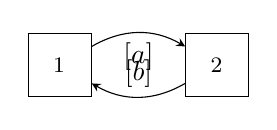
\begin{tikzpicture}[node distance=1.5cm,scale=1]
        \node (square-h) [draw,minimum width=0.8cm,minimum height=0.8cm] {\large $\hh_1$};
        \node (square-k) [draw,minimum width=0.8cm,minimum height=0.8cm, right of = square-h, xshift=5mm] {\large $\hh_2$};
       % 
      \path
      (square-h) edge[-stealth,bend left] node[below] {$\msg[a]$} (square-k)
      (square-k) edge[-stealth,bend left] node[above] {$\msg[b]$} (square-h)
      ;
 \end{tikzpicture}
 }
 %
 \hspace{8mm}
 %
\begin{array}{l}
\text{$\cs_2$}\\[12mm]
\end{array}
 \dbox{
 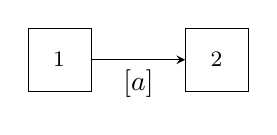
\begin{tikzpicture}[node distance=1.5cm,scale=1]
        \node (square-h) [draw,minimum width=0.8cm,minimum height=0.8cm] {\large $\hh_1$};
        \node (square-k) [draw,minimum width=0.8cm,minimum height=0.8cm, right of = square-h, xshift=5mm] {\large $\hh_2$};
       % 
      \path
      (square-h) edge[-stealth] node[below] {$\msg[a]$} (square-k)
      ;
 \end{tikzpicture} 
        }
 %
 \hspace{8mm}
 %
\begin{array}{l}
\text{$\cs_3$}\\[12mm]
\end{array}
 \dbox{
 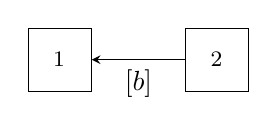
\begin{tikzpicture}[node distance=1.5cm,scale=1]
        \node (square-h) [draw,minimum width=0.8cm,minimum height=0.8cm] {\large $\hh_1$};
        \node (square-k) [draw,minimum width=0.8cm,minimum height=0.8cm, right of = square-h, xshift=5mm] {\large $\hh_2$};
       % 
      \path
      (square-k) edge[-stealth] node[below] {$\msg[b]$} (square-h)
      ;
 \end{tikzpicture} 
        }
 \end{equation}
%  $
% \caption{\label{fig:pcm} Three connection models for composing the systems in \cref{fig:twoipnterfaces}}
% }
%\end{figure}

Notice that the connection models depends only on the choosen interface interactions.
This holds however only for the binary case.
Not for the multicomposition (see below).

The following partial gateways can be obtained out of the interface participants and the connection
models.
\begin{equation}
\hspace{-8mm}
\begin{tikzpicture}[node distance=1.5cm,scale=1]
        \node (square-v)  [draw,minimum width=0.8cm,minimum height=0.8cm] {\large $\hh_3$};
        \node [state] (v-b) [left of = square-v, draw=none] {};
        \node [state] (v-a) [below of = square-v, draw=none] {};
        \draw [-stealth] (v-a) --  node {$\msg[a]$} (square-v);
        \draw [-stealth] (square-v) --  node {$\msg[b]$} (v-b);
        \node (square-w)  [draw,minimum width=0.8cm,minimum height=0.8cm, right of = square-v] {\large $\hh_4$};
        \node [state] (w-c) [right of = square-w, draw=none] {};
        \node [state] (w-a) [below of = square-w, draw=none] {};
        \node [state] (w-b) [above right of = square-w, draw=none] {};
        \draw [-stealth] (w-c) --  node {$\msg[c]$} (square-w);
        \draw [-stealth] (square-w) --  node {$\msg[a]$} (w-a);
        \draw [stealth-] (square-w) --  node {$\msg[b]$} (w-b);
        %
        \draw [-stealth] (square-w) to[out=-135,in=-45]  node {$\msg[b]$} (square-v);
        %
        \draw (0.4,0)[dotted,thick]  --  (0,-0.4); % carrying a inside v
        \draw (0.4,-0.4)[dotted,thick]  --  (-0.4,0); % carrying b inside v
        %
        \draw (1.5,0.4)[dotted,thick]  --  (1.5,-0.4); % carrying a inside w
        \draw (1.1,-0.4)[dotted,thick]  to[out=30,in=260]  (1.9,0.4); % carrying b inside w
        %
        %
        \draw [-stealth]  (0.4,0) to[out=45,in=90]  node [pos=0.6] {$\msg[a]$} (1.5,0.4 ); % carryng a from v to w  
 \end{tikzpicture}
 \hspace{0mm}
 \begin{tikzpicture}[node distance=1.5cm,scale=1]
        \node (square-v)  [draw,minimum width=0.8cm,minimum height=0.8cm] {\large $\hh_3$};
        \node [state] (v-b) [left of = square-v, draw=none] {};
        \node [state] (v-a) [below of = square-v, draw=none] {};
        \draw [-stealth] (v-a) --  node {$\msg[a]$} (square-v);
        \draw [-stealth] (square-v) --  node {$\msg[b]$} (v-b);
        \node (square-w)  [draw,minimum width=0.8cm,minimum height=0.8cm, right of = square-v] {\large $\hh_4$};
        \node [state] (w-c) [right of = square-w, draw=none] {};
        \node [state] (w-a) [below of = square-w, draw=none] {};
        \node [state] (w-b) [above right of = square-w, draw=none] {};
        \draw [-stealth] (w-c) --  node {$\msg[c]$} (square-w);
        \draw [-stealth] (square-w) --  node {$\msg[a]$} (w-a);
        \draw [stealth-] (square-w) --  node {$\msg[b]$} (w-b);
        %
        \draw [-stealth] (square-w) to[out=-135,in=-45]  node {$\msg[b]$} (square-v);
        %
        %\draw (0.4,0)[dotted,thick]  --  (0,-0.4); % carrying a inside v
        \draw (0.4,-0.4)[dotted,thick]  --  (-0.4,0); % carrying b inside v
        %
        %\draw (1.5,0.4)[dotted,thick]  --  (1.5,-0.4); % carrying a inside w
        \draw (1.1,-0.4)[dotted,thick]  to[out=30,in=260]  (1.9,0.4); % carrying b inside w
        %
        %
       % \draw [-stealth]  (0.4,0) to[out=45,in=90]  node [pos=0.6] {$\msg[a]$} (1.5,0.4 ); % carryng a from v to w  
 \end{tikzpicture}
 \hspace{0mm}
\begin{tikzpicture}[node distance=1.5cm,scale=1]
        \node (square-v)  [draw,minimum width=0.8cm,minimum height=0.8cm] {\large $\hh_3$};
        \node [state] (v-b) [left of = square-v, draw=none] {};
        \node [state] (v-a) [below of = square-v, draw=none] {};
        \draw [-stealth] (v-a) --  node {$\msg[a]$} (square-v);
        \draw [-stealth] (square-v) --  node {$\msg[b]$} (v-b);
        \node (square-w)  [draw,minimum width=0.8cm,minimum height=0.8cm, right of = square-v] {\large $\hh_4$};
        \node [state] (w-c) [right of = square-w, draw=none] {};
        \node [state] (w-a) [below of = square-w, draw=none] {};
        \node [state] (w-b) [above right of = square-w, draw=none] {};
        \draw [-stealth] (w-c) --  node {$\msg[c]$} (square-w);
        \draw [-stealth] (square-w) --  node {$\msg[a]$} (w-a);
        \draw [stealth-] (square-w) --  node {$\msg[b]$} (w-b);
        %
        %\draw [-stealth] (square-w) to[out=-135,in=-45]  node {$\msg[b]$} (square-v);
        %
        \draw (0.4,0)[dotted,thick]  --  (0,-0.4); % carrying a inside v
        %\draw (0.4,-0.4)[dotted,thick]  --  (-0.4,0); % carrying b inside v
        %
        \draw (1.5,0.4)[dotted,thick]  --  (1.5,-0.4); % carrying a inside w
        %
        %
        \draw [-stealth]  (0.4,0) to[out=45,in=90]  node [pos=0.6] {$\msg[a]$} (1.5,0.4 ); % carryng a from v to w  
 \end{tikzpicture}
\end{equation}




This approach to composition easily scales up to general multiple composition. 

Let us consider an example from~\cite{BDGY23} having four systems $S_1$,  $S_2$, $S_3$ and $S_4$.
As shown in (\ref{eq:four-ips}) below, we have selected for each system one participant
as an interface, named respectively $\hh_1$, $\hh_2$, $\hh_3$ and $\hh_4$.
 
%\begin{wrapfigure}{r}{0.45\textwidth}
%\begin{figure}[h]
%    %\vspace{-8mm}
%     \centering{\small
%    $
\begin{equation}
\label{eq:four-ips}
    \begin{array}{@{\hspace{0mm}}c@{\hspace{-2mm}}}
    \begin{array}{c@{\hspace{-2mm}}c}
    \text{\large $S_1$}
    &
 \begin{tikzpicture}[node distance=1.5cm,scale=1]
        \node (square-h) [draw,minimum width=0.8cm,minimum height=0.8cm] {\large $\hh_1$};
        \node [state] (h-a) [above of = square-h, draw=none] {};
        \node [state] (h-c) [left of = square-h, draw=none] {};
        \draw [-stealth] (h-a) --  node {$\msg[a]$} (square-h);
        \draw [-stealth] (square-h) --  node {$\msg[c]$} (h-c);
 \end{tikzpicture}
 \end{array}
 \hspace{4mm}
\begin{array}{c}
 \\
 \\
| \\
| \\
|\\
|\\
\end{array}
 \hspace{4mm}
 \begin{array}{c@{\hspace{-2mm}}c}
\begin{tikzpicture}[node distance=1.5cm,scale=1]
        \node (square-k) [draw,minimum width=0.8cm,minimum height=0.8cm] {\large $\hh_2$};
        \node [state] (k-b) [above of = square-k, draw=none] {};
        \node [state] (k-a) [right of = square-k, draw=none] {};
        \draw [-stealth] (k-b) --  node {$\msg[b]$} (square-k);
        \draw [-stealth] (square-k) --  node {$\msg[a]$} (k-a);
 \end{tikzpicture}
 &
 \text{\large $S_2$} 
 \end{array}
 \\[12mm]
\hspace{3mm}- - - -    \hspace{8mm}- - - - -  \\[-5mm]
\begin{array}{@{\hspace{0mm}}c@{\hspace{0mm}}c}
\\[4mm]
\text{\large $S_3\hspace{-2mm}$} 
&
 \begin{tikzpicture}[node distance=1.5cm,scale=1]
        \node (square-v) [draw,minimum width=0.8cm,minimum height=0.8cm] {\large $\hh_3$};
        \node [state] (v-b) [left of = square-v, draw=none] {};
        \node [state] (v-a) [below of = square-v, draw=none] {};
        \draw [-stealth] (v-a) --  node {$\msg[a]$} (square-v);
        \draw [-stealth] (square-v) --  node {$\msg[b]$} (v-b);
 \end{tikzpicture}
 \end{array}
 \hspace{4mm}
\begin{array}{c}
 \\[-8mm]
| \\
| \\
| \\
|
\end{array}
 \hspace{4mm}
 \begin{array}{c@{\hspace{-2mm}}}
 \\[-6mm]
 \begin{tikzpicture}[node distance=1.5cm,scale=1]
        \node (square-w) [draw,minimum width=0.8cm,minimum height=0.8cm] {\large $\hh_4$};
        \node [state] (w-c) [right of = square-w, draw=none] {};
        \node [state] (w-a) [below of = square-w, draw=none] {};
        \node [state] (w-b) [above right of = square-w, draw=none] {};
        \draw [-stealth] (w-c) --  node {$\msg[c]$} (square-w);
        \draw [-stealth] (square-w) --  node {$\msg[a]$} (w-a);
        \draw [stealth-] (square-w) --  node {$\msg[b]$} (w-b);
 \end{tikzpicture}
 \hspace{-6mm}
 \begin{array}{l}
 \\[6mm]
 \text{\large\ \ $S_4$}
 \end{array} 
 \end{array}
 \\[-4mm]
 \end{array}
 \end{equation}
% $
% }
%\caption{\label{fig:four-ips}
%Four systems with their respective interface participants}
% \end{figure}
% \vspace{-5mm}
% \end{wrapfigure}

We could take into account the following interface actions.

%\begin{figure}[h]
%    %\vspace{-8mm}
%     \centering{\small
%    $
\begin{equation}
\label{eq:four-ips}
    \begin{array}{@{\hspace{0mm}}c@{\hspace{-2mm}}}
    \begin{array}{c@{\hspace{-2mm}}c}
    \text{\large $S_1$}
    &
 \begin{tikzpicture}[node distance=1.5cm,scale=1]
        \node (square-h) [draw,minimum width=0.8cm,minimum height=0.8cm] {\large $\hh_1$};
        \node [state] (h-a) [above of = square-h, draw=none] {};
        \node [state] (h-c) [left of = square-h, draw=none] {};
        \draw [-stealth,line width=0.5mm] (h-a) --  node [right] {$\msg[a]$} (square-h);
        \draw [-stealth] (square-h) --  node {$\msg[c]$} (h-c);
 \end{tikzpicture}
 \end{array}
 \hspace{4mm}
\begin{array}{c}
 \\
 \\
| \\
| \\
|\\
|\\
\end{array}
 \hspace{4mm}
 \begin{array}{c@{\hspace{-2mm}}c}
\begin{tikzpicture}[node distance=1.5cm,scale=1]
        \node (square-k) [draw,minimum width=0.8cm,minimum height=0.8cm] {\large $\hh_2$};
        \node [state] (k-b) [above of = square-k, draw=none] {};
        \node [state] (k-a) [right of = square-k, draw=none] {};
        \draw [-stealth, line width=0.5mm] (k-b) --  node [right] {$\msg[b]$} (square-k);
        \draw [-stealth, line width=0.5mm] (square-k) --  node [below] {$\msg[a]$} (k-a);
 \end{tikzpicture}
 &
 \text{\large $S_2$} 
 \end{array}
 \\[12mm]
\hspace{3mm}- - - -    \hspace{8mm}- - - - -  \\[-5mm]
\begin{array}{@{\hspace{0mm}}c@{\hspace{0mm}}c}
\\[4mm]
\text{\large $S_3\hspace{-2mm}$} 
&
 \begin{tikzpicture}[node distance=1.5cm,scale=1]
        \node (square-v) [draw,minimum width=0.8cm,minimum height=0.8cm] {\large $\hh_3$};
        \node [state] (v-b) [left of = square-v, draw=none] {};
        \node [state] (v-a) [below of = square-v, draw=none] {};
        \draw [-stealth,line width=0.5mm] (v-a) --  node [right]   {$\msg[a]$} (square-v);
        \draw [-stealth,line width=0.5mm] (square-v) --  node [below] {$\msg[b]$} (v-b);
 \end{tikzpicture}
 \end{array}
 \hspace{4mm}
\begin{array}{c}
 \\[-8mm]
| \\
| \\
| \\
|
\end{array}
 \hspace{4mm}
 \begin{array}{c@{\hspace{-2mm}}}
 \\[-6mm]
 \begin{tikzpicture}[node distance=1.5cm,scale=1]
        \node (square-w) [draw,minimum width=0.8cm,minimum height=0.8cm] {\large $\hh_4$};
        \node [state] (w-c) [right of = square-w, draw=none] {};
        \node [state] (w-a) [below of = square-w, draw=none] {};
        \node [state] (w-b) [above right of = square-w, draw=none] {};
        \draw [-stealth] (w-c) --  node {$\msg[c]$} (square-w);
        \draw [-stealth,line width=0.5mm] (square-w) --  node [right] {$\msg[a]$} (w-a);
        \draw [stealth-] (square-w) --  node {$\msg[b]$} (w-b);
 \end{tikzpicture}
 \hspace{-6mm}
 \begin{array}{l}
 \\[6mm]
 \text{\large\ \ $S_4$}
 \end{array} 
 \end{array}
 \\[-4mm]
 \end{array}
 \end{equation}
% $
% }
%\caption{\label{fig:four-ips}
%Four interfaces with particular interface actions.}
% \end{figure}
% \vspace{-5mm}
% \end{wrapfigure}

Unlike the binary case, a connection policy is not uniquely determined the specification
of which are the interface actions in the interface participants.

For what concerns  the choice of interface actions highlighted in (\ref{eq:four-ips}),
 one could decide that message $\msg[a]$ received by $\hh_1$ has 
 to be forwarded
 to $\hh_4$; the $\msg[a]$ received by $\hh_3$
 to $\hh_2$; the $\msg[b]$ received by $\hh_2$ to $\hh_3$.
 Another possible choice 
could be similar to the previous one but for the forwarding
of the messages $\msg[a]$: the one received by $\HH_1$ could be forwarded now to $\hh_2$
whereas the one received by $\hh_3$ could be forwarded to $\hh_4$. 
So, it is possible to have the following two connection models, both coherent
with the interface actions highlighted in (\ref{fig:four-ips}).  
 

%%% CONNECTION MODELS
% \begin{figure}[ht]
%    \centering{
 \begin{equation}
    \raisebox{15mm}{$\cs_\mathrm{A}$}
    \begin{array}{c@{\qquad\qquad\qquad\qquad\qquad}c}
\dbox{
 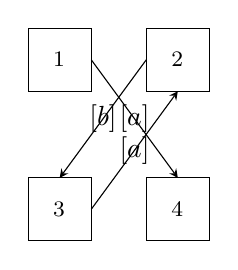
\begin{tikzpicture}[node distance=1.5cm,scale=1]
        \node (square-h) [draw,minimum width=0.8cm,minimum height=0.8cm] {\large $\hh_1$};
        \node (square-k) [draw,minimum width=0.8cm,minimum height=0.8cm, right of = square-h] {\large $\hh_2$};
        \node (square-v)  [draw,minimum width=0.8cm,minimum height=0.8cm, below of = square-h, yshift=-4mm] {\large $\hh_3$};
        \node (square-w)  [draw,minimum width=0.8cm,minimum height=0.8cm, below of = square-k, yshift=-4mm] {\large $\hh_4$};
        %\draw[-stealth]  (square-w) to[out=-135,in=-45]  node {$\msg[b]$} (square-v);
        %
        %
        \draw [-stealth] (0.4,0)  -- node {$\msg[a]$}  (1.5,-1.5 ); % carryng a from h to w    
        % \draw [stealth-] (0,-0.4)  -- node {$\msg[c]$} (1.1,-1.9); % carryng c from w to h 
        \draw [-stealth] (0.4,-1.9)  --  node {$\msg[a]$} (1.5,-0.4 ); % carrying a from v to k
        \draw [stealth-] (0,-1.5)  --  node {$\msg[b]$} (1.1,0); % carrying  b from k to v
 \end{tikzpicture}
 }
&
\dbox{
 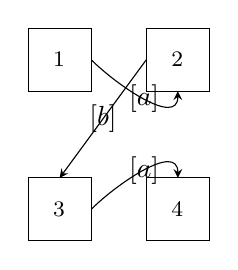
\begin{tikzpicture}[node distance=1.5cm,scale=1]
        \node (square-h) [draw,minimum width=0.8cm,minimum height=0.8cm] {\large $\HH_1$};
        \node (square-k) [draw,minimum width=0.8cm,minimum height=0.8cm, right of = square-h] {{\large $\hh_2$}};
        \node (square-v)  [draw,minimum width=0.8cm,minimum height=0.8cm, below of = square-h, yshift=-4mm] {{\large $\hh_3$}};
        \node (square-w)  [draw,minimum width=0.8cm,minimum height=0.8cm, below of = square-k, yshift=-4mm] {{\large $\hh_4$}};
        %
        %\draw [-stealth] (square-w) to[out=-135,in=-45]  node {$\msg[b]$} (square-v);
        %
        %
        \draw [-stealth] (0.4,-1.9) to[out=45,in=90] node {$\msg[a]$} (1.5,-1.5 ); % carryng a from v to w    
         %\draw [stealth-] (0,-0.4)  -- node {$\msg[c]$} (1.1,-1.9) ; % carryng c from w to h 
        \draw [-stealth]  (0.4,0)  to[out=-45,in=-90]  node {$\msg[a]$} (1.5,-0.4 ); % carrying a from h to k
        %\draw [-stealth]  (square-v)  to[out=45,in=-90]  node {$\msg[a]$} (square-k); % carrying a from h to k
        \draw [stealth-] (0,-1.5)  --  node {$\msg[b]$} (1.1,0); % carrying  b from k to v
 \end{tikzpicture}
 }
 \raisebox{14.5mm}{$\,\,\,\,\cs_\mathrm{B}$}
 \end{array}
  \end{equation}
% $
% }
% \caption{\label{fig:choicesAB} Two connection models for multicomposition.}\label{fig:twocm}
% \end{figure}
 
 \noindent
  Similarly to the binary case, the PaI multicomposition via partial gateways of the four
 systems consists in fact in replacing the participants  $\hh_1$, $\hh_2$, $\hh_3$ and $\hh_4$, chosen  as
interfaces, by gateways whose task stays the same for what concerns the non interface-actions,
whereas messages of interfaces actions are simply forwarded.
 The  architecture  of the resulting composed systems, according to the connection models is
represented  by the diagrams  in (\ref{eq:multiconnection}),  where the names $\hh_1, \hh_2, \hh_3$
and $\hh_4$ are now partial gateways.
%\begin{figure}[h]%{c}{0.6\textwidth}
%\vspace{-4mm}
%    \centering{
\vspace{-4mm} 
\begin{equation}
 \label{eq:multiconnection}
    \begin{array}{c@{\quad\qquad}c}
 \begin{tikzpicture}[node distance=1.5cm,scale=1]
        \node (square-h) [draw,minimum width=0.8cm,minimum height=0.8cm] {\large $\hh_1$};
        \node [state] (h-a) [above of = square-h, draw=none] {};
        \node [state] (h-c) [left of = square-h, draw=none] {};
        \draw [-stealth] (h-a) --  node {$\msg[a]$} (square-h);
        \draw [-stealth] (square-h) --  node {$\msg[c]$} (h-c);
        \node (square-k) [draw,minimum width=0.8cm,minimum height=0.8cm, right of = square-h] {\large $\hh_2$};
        \node [state] (k-b) [above of = square-k, draw=none] {};
        \node [state] (k-a) [right of = square-k, draw=none] {};
        \draw [-stealth] (k-b) --  node {$\msg[b]$} (square-k);
        \draw [-stealth] (square-k) --  node {$\msg[a]$} (k-a);
        \node (square-v)  [draw,minimum width=0.8cm,minimum height=0.8cm, below of = square-h, yshift=-4mm] {\large $\hh_3$};
        \node [state] (v-b) [left of = square-v, draw=none] {};
        \node [state] (v-a) [below of = square-v, draw=none] {};
        \draw [-stealth] (v-a) --  node {$\msg[a]$} (square-v);
        \draw [-stealth] (square-v) --  node {$\msg[b]$} (v-b);
        \node (square-w)  [draw,minimum width=0.8cm,minimum height=0.8cm, below of = square-k, yshift=-4mm] {\large $\hh_4$};
        \node [state] (w-c) [right of = square-w, draw=none] {};
        \node [state] (w-a) [below of = square-w, draw=none] {};
        \node [state] (w-b) [above right of = square-w, draw=none] {};
        \draw [-stealth] (w-c) --  node {$\msg[c]$} (square-w);
        \draw [-stealth] (square-w) --  node {$\msg[a]$} (w-a);
        \draw [stealth-] (square-w) --  node {$\msg[b]$} (w-b);
        %
      %  \draw (square-h)  to[out=-90,in=90]   node {} (square-w);
       % \draw (square-k) to[out=-90,in=90]  node {} (square-v);
      %  \draw (square-h) to[out=0,in=180]  node {} (square-w);
      %  \draw [-stealth] (square-w) to[out=-135,in=-45]  node {$\msg[b]$} (square-v);
      %  \draw (square-k) to[out=-135,in=45]  node {} (square-v);
        %
        \draw (0,0.4)[dotted,thick]  --  (0.4,0); % carrying a inside h  
        %\draw (-0.4,0)[dotted,thick]  --  (0,-0.4); % carrying c inside h
        %
        \draw (1.5,0.4)[dotted,thick]  --  (1.1,0); % carrying b inside k
        \draw (1.5,-0.4)[dotted,thick]  --  (1.9,0); % carrying a inside k
        %
        \draw (0.4,-1.9)[dotted,thick]  --  (0,-2.3); % carrying a inside v
        \draw (0,-1.5)[dotted,thick]  --  (-0.4,-1.9); % carrying k's b inside v
        %\draw (0.4,-2.3)[dotted,thick]  --  (-0.4,-1.9); % carrying b inside v
        %
        \draw (1.5,-1.5)[dotted,thick]  --  (1.5,-2.3); % carrying a inside w
        %\draw (1.1,-1.9)[dotted,thick]  --  (1.9,-1.9); % carrying c inside w
        %\draw (1.1,-2.3)[dotted,thick]  to[out=30,in=260]  (1.9,-1.5); % carrying b inside w
        %
        %
        \draw[-stealth]   (0.4,0)  -- node  {$\msg[a]$}   (1.5,-1.5 ); % carryng a from h to w    
         %\draw  [stealth-]  (0,-0.4)  --  node  {$\msg[c]$}  (1.1,-1.9); % carryng c from w to h 
        \draw [-stealth]  (0.4,-1.9)  --   node  {$\msg[a]$} (1.5,-0.4 ); % carrying a from v to k
        \draw [stealth-]  (0,-1.5)  --  node {$\msg[b]$} (1.1,0); % carrying  b from k to v
 \end{tikzpicture}
& 
\begin{tikzpicture}[node distance=1.5cm,scale=1]
        \node (square-h) [draw,minimum width=0.8cm,minimum height=0.8cm] {\large $\HH$};
        \node [state] (h-a) [above of = square-h, draw=none] {};
        \node [state] (h-c) [left of = square-h, draw=none] {};
        \draw [-stealth] (h-a) --  node {$\msg[a]$} (square-h);
        \draw [-stealth] (square-h) --  node {$\msg[c]$} (h-c);
        \node (square-k) [draw,minimum width=0.8cm,minimum height=0.8cm, right of = square-h] {\large $\KK$};
        \node [state] (k-b) [above of = square-k, draw=none] {};
        \node [state] (k-a) [right of = square-k, draw=none] {};
        \draw [-stealth] (k-b) --  node {$\msg[b]$} (square-k);
        \draw [-stealth] (square-k) --  node {$\msg[a]$} (k-a);
        \node (square-v)  [draw,minimum width=0.8cm,minimum height=0.8cm, below of = square-h, yshift=-4mm] {\large $\hh_3$};
        \node [state] (v-b) [left of = square-v, draw=none] {};
        \node [state] (v-a) [below of = square-v, draw=none] {};
        \draw [-stealth] (v-a) --  node {$\msg[a]$} (square-v);
        \draw [-stealth] (square-v) --  node {$\msg[b]$} (v-b);
        \node (square-w)  [draw,minimum width=0.8cm,minimum height=0.8cm, below of = square-k, yshift=-4mm] {\large $\hh_4$};
        \node [state] (w-c) [right of = square-w, draw=none] {};
        \node [state] (w-a) [below of = square-w, draw=none] {};
        \node [state] (w-b) [above right of = square-w, draw=none] {};
        \draw [-stealth] (w-c) --  node {$\msg[c]$} (square-w);
        \draw [-stealth] (square-w) --  node {$\msg[a]$} (w-a);
        \draw [stealth-] (square-w) --  node {$\msg[b]$} (w-b);
        %
        %\draw [-stealth] (square-w) to[out=-135,in=-45]  node {$\msg[b]$} (square-v);
        %
        \draw (0,0.4)[dotted,thick]  --  (0.4,0); % carrying a inside h  
        %\draw (-0.4,0)[dotted,thick]  --  (0,-0.4); % carrying c inside h
        %
        \draw (1.5,0.4)[dotted,thick]  --  (1.1,0); % carrying b inside k
        \draw (1.5,-0.4)[dotted,thick]  --  (1.9,0); % carrying a inside k
        %
        \draw (0.4,-1.9)[dotted,thick]  --  (0,-2.3); % carrying a inside v
        \draw (0,-1.5)[dotted,thick]  --  (-0.4,-1.9); % carrying k's b inside v
        %\draw (0.4,-2.3)[dotted,thick]  --  (-0.4,-1.9); % carrying b inside v
        %
        \draw (1.5,-1.5)[dotted,thick]  --  (1.5,-2.3); % carrying a inside w
        %\draw (1.1,-1.9)[dotted,thick]  --  (1.9,-1.9); % carrying c inside w
        %\draw (1.1,-2.3)[dotted,thick]  to[out=30,in=260]  (1.9,-1.5); % carrying b inside w
        %
        %
        \draw [-stealth]  (0.4,-1.9) to[out=45,in=90]  node [pos=0.6] {$\msg[a]$} (1.5,-1.5 ); % carryng a from v to w    
         %\draw [stealth-]  (0,-0.4)  --  node  {$\msg[c]$} (1.1,-1.9); % carryng c from w to h 
        \draw [-stealth]  (0.4,0)  to[out=-45,in=-90]  node [pos=0.6]  {$\msg[a]$} (1.5,-0.4 ); % carrying a from h to k
        \draw [stealth-]  (0,-1.5)  -- node  {$\msg[b]$}  (1.1,0); % carrying  b from k to v
 \end{tikzpicture}\\[-4mm]
 \text{\small (Using $\cs_\mathrm{A}$)}
 &
 \text{\small (Using $\cs_\mathrm{B}$)}
 \end{array}
  \end{equation}
 
%  }
%  \vspace{-1mm}
%  \caption{Static description of two PaI multicompositions via partial gateways}
%  \label{fig:multiconnection}
% \end{figure}

One of the main results of the paper is that a number of comminication properties
are preserved by PaI multicomposition via partial gateways in case the very same
properties are enjoied by the connection policy used for the composition.
Such a result is actually obtained as a corollary of a preservation result for 
a restricted form of binary PaI composition that we dub partial-fusion PaI composition.
All forms of PaI composition for asynchronous CFSM can be obtained by a number
of binary partial-fusion PaI composition, which can hence be considered as the 
basis of the PaI approach.

\paragraph{Partial Fusion PaI Composition}

This particular form of PaI composition is binary.
To get an intuitive idea of that, let us consider the following simple example, where
both $S_1$ and $S_2$ possess a participant named $\hh$ that we choose as
their respective interface participant.

\begin{equation}
\label{eq:exps}
\raisebox{2mm}{\text{\large $S_1$}\,\,}
%    \dbox{
\hspace{10mm} \begin{tikzpicture}[node distance=1.5cm,scale=1]
        \node (square-h) [draw,minimum width=0.8cm,minimum height=0.8cm] {\large $\hh$};
        \node [state] (h-a) [above of = square-h, draw=none] {};
        \node [state] (h-c) [left of = square-h, draw=none, xshift=-2mm] {};
        \draw [-stealth] (h-a) --  node {$\msg[a]$} (square-h);
        \draw [stealth-] (h-c) --  node {$\msg[b]$} (square-h);
 \end{tikzpicture}
%            }
\hspace{2mm}
 \begin{array}{c}
 \\[8mm]
| \\
| \\
|\\
|\\
\end{array}
\hspace{4mm}
%     \dbox{
 \begin{tikzpicture}[node distance=1.5cm,scale=1]
        \node (square-k) [draw,minimum width=0.8cm,minimum height=0.8cm] {\large $\hh$};
        \node [state] (k-b) [above of = square-k, draw=none] {};
        \node [state] (k-a) [right of = square-k, draw=none] {};
        %\draw [stealth-] (k-b) --  node[right] {$\msg[inf]$} (square-k);
        \draw [-stealth] (square-k) --  node {$\msg[a]$} (k-a);
       % \draw  [-stealth] (0.4,-0.2)   --  node [below] {$\msg[par]$} (1.2,-0.2);
 \end{tikzpicture} \hspace{18mm}
 %            }
 \raisebox{0mm}{\text{\large $\,\,S_2$}}
 \end{equation}
 
The composition method requires that some interaction actions are choosen in only one
of the two interface participants.  

\begin{equation}
\label{eq:expsia}
\begin{array}{c}
\\[-18mm]
\raisebox{2mm}{\text{\large $S_1$}\,\,}
%    \dbox{
\hspace{10mm} \begin{tikzpicture}[node distance=1.5cm,scale=1]
        \node (square-h) [draw,minimum width=0.8cm,minimum height=0.8cm] {\large $\hh$};
        \node [state] (h-a) [above of = square-h, draw=none] {};
        \node [state] (h-c) [left of = square-h, draw=none, xshift=-2mm] {};
        \draw [-stealth,line width=0.5mm] (h-a) --  node[right] {$\msg[a]$} (square-h);
        \draw [stealth-] (h-c) --  node {$\msg[b]$} (square-h);
 \end{tikzpicture}
%            }
\hspace{2mm}
 \begin{array}{c}
 \\[8mm]
| \\
| \\
|\\
|\\
\end{array}
\hspace{4mm}
%     \dbox{
 \begin{tikzpicture}[node distance=1.5cm,scale=1]
        \node (square-k) [draw,minimum width=0.8cm,minimum height=0.8cm] {\large $\hh$};
        \node [state] (k-b) [above of = square-k, draw=none] {};
        \node [state] (k-a) [right of = square-k, draw=none] {};
        %\draw [stealth-] (k-b) --  node[right] {$\msg[inf]$} (square-k);
        \draw [-stealth] (square-k) --  node {$\msg[a]$} (k-a);
       % \draw  [-stealth] (0.4,-0.2)   --  node [below] {$\msg[par]$} (1.2,-0.2);
 \end{tikzpicture} \hspace{18mm}
 %            }
 \raisebox{0mm}{\text{\large $\,\,S_2$}}
 \end{array}
 \end{equation}

We ``restrict'' now the behaviour of  $\hh$ in $S_1$ (the interface participant with interface actions)
to its interface actions only.
\begin{equation}
\begin{array}{c}
\\[-18mm]
\begin{tikzpicture}[node distance=1.5cm,scale=1]
        \node (square-h) [draw,minimum width=0.8cm,minimum height=0.8cm] {\large $\hh'$};
        \node [state] (h-a) [above of = square-h, draw=none] {};
        \node [state] (h-c) [left of = square-h, draw=none, xshift=-2mm] {};
        \draw [-stealth] (h-a) --  node {$\msg[a]$} (square-h);
 \end{tikzpicture}
  \end{array}
\end{equation}

The composition can be carried on now, since $\hh'$ above and $\hh$ of $S_2$ in (\ref{eq:expsia}) 
are dual (one has an input where the other has an output end vice versa).
 Such a duality property enables to (partially) fuse together the $\hh$ in $S_1$ with the
 $\hh$ in $S_2$ so obtaining a composed system.
 The fusion makes $h$ a single gateway forwarding the messages pertaining to
 interface actions and behaving as $\hh$ of $S_1$ for the non interface-actions.

\begin{equation}
\label{fig:bincomp}
\begin{array}{l}
\text{\large $S_1$}\!\stackrel{\hh_1{\leftrightarrow}\hh_2}{ \phantom{\mathtt{comp}}}\text{\large $S_2$}\\[22mm]
\end{array}
 \dbox{ \hspace{28mm}
 \begin{tikzpicture}[node distance=1.5cm,scale=1]
        \node (square-h) [draw,minimum width=0.8cm,minimum height=0.8cm] {\large $\hh_1$};
        \draw [-stealth] (h-a) --  node [right] {$\msg[sbs]$} (square-h);
         \node[draw=none,fill=none] (phantom2) [left = 10mm  of square-h]{};
        \draw [-stealth] (square-k) --  node [above]{$\msg[sbs]$} (k-a);
        \draw [stealth-] (phantom2) --  node [above]{$\msg[inf]$} (square-h);
         %
        \draw (0,0.4)[dotted,thick]  --  (0.4,0); % carrying sbs inside h 
        \draw (-0.4,0)[dotted,thick]  --  (0.4,-0.2); % carrying par inside h 
        \draw [-stealth] (0.4,0)  --  (1.6,0); % carrying sbs from h1 to h2
        \draw [stealth-] (0.4,-0.2)  --  (1.6,-0.2); % carrying inf from h1 to h2
        \draw (1.6,-0.2) [dotted,thick]  --  (2.4,-0.2); % carrying inf inside h2
        \draw  [stealth-] (2.4,-0.2)   --  node [below] {$\msg[inf]$} (3.25,-0.2); % carrying inf outside h2
        \draw (1.6,0)[dotted,thick]  --  (2.4,0); % carrying sbs inside h2
 \end{tikzpicture}
       }
\end{equation}

In the binary case the connection policy for \cref{fig:twoipnterfaces} is uniquely determined, and
abstracting from choices and dynamic aspects can be represented by the following 
system with two participants.

%\begin{figure}[h]
%    \centering{\small
%    $
\begin{equation}
\label{fig:pcp}
\begin{array}{l}
\text{$\cs$}\\[12mm]
\end{array}
 \dbox{
 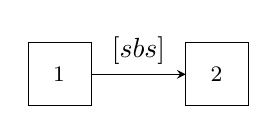
\begin{tikzpicture}[node distance=1.5cm,scale=1]
        \node (square-h) [draw,minimum width=0.8cm,minimum height=0.8cm] {\large $\hh_1$};
        \node (square-k) [draw,minimum width=0.8cm,minimum height=0.8cm, right of = square-h, xshift=5mm] {\large $\hh_2$};
         %
        \draw [-stealth] (0.4,0)  --  node [above] {$\msg[sbs]$} (1.6,0); % carrying sbs from h1 to h2 h2
 \end{tikzpicture}
 }
 \end{equation}
% $
% \caption{\label{fig:pcp} A connection policy for composing the systems in \cref{fig:twoipnterfaces}}
% }
%\end{figure}

The partial gateways of \cref{fig:binpcomp} can be built out of  $\hh_1$ and $\hh_2$ in 
\cref{fig:twoipnterfaces} and the connection policy $\cs$ in \cref{fig:pcp}.

As a matter of fact, the system of \label{fig:binpcomp} can be obtained by 
means of two different composition of a restricted kind (fusion).

% \begin{figure}[h]
%    \centering{\small
%    $
\begin{equation}
\label{fig:twoipnterfaces}
\raisebox{10mm}{\text{\large $S_1$}\,\,}
    \dbox{
\hspace{10mm} \begin{tikzpicture}[node distance=1.5cm,scale=1]
        \node (square-h) [draw,minimum width=0.8cm,minimum height=0.8cm] {\large $\hh_1$};
        \node [state] (h-a) [above of = square-h, draw=none] {};
        \node [state] (h-c) [left of = square-h, draw=none, xshift=-2mm] {};
        \draw [-stealth] (h-a) --  node[right] {$\msg[sbs]$} (square-h);
        \draw [stealth-] (h-c) --  node[above] {$\msg[inf]$} (square-h);
 \end{tikzpicture}
            }
\hspace{12mm}
 \begin{array}{l}
\text{$\cs$}\\[12mm]
\end{array}
 \dbox{
 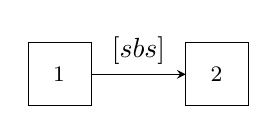
\begin{tikzpicture}[node distance=1.5cm,scale=1]
        \node (square-h) [draw,minimum width=0.8cm,minimum height=0.8cm] {\large $\hh_1$};
        \node (square-k) [draw,minimum width=0.8cm,minimum height=0.8cm, right of = square-h, xshift=5mm] {\large $\hh_2$};
         %
        \draw [-stealth] (0.4,0)  --  node [above] {$\msg[sbs]$} (1.6,0); % carrying sbs from h1 to h2 h2
 \end{tikzpicture}
 }
 \end{equation}
% $\vspace{-2mm}
% \caption{\label{fig:twoipnterfaces} Two interfaces participants belonging to, respectively, systems $S_1$ and $S_2$.}
% }
%\end{figure}

%\begin{figure}[h]
%    \centering{\small
%    $
\begin{equation}
\label{fig:binpcomp}
\begin{array}{l}
\text{\large $S_1$}\!\mathtt{fused}\text{$\cs$}\\[22mm]
\end{array}
 \dbox{ \hspace{28mm}
 \begin{tikzpicture}[node distance=1.5cm,scale=1]
        \node (square-h) [draw,minimum width=0.8cm,minimum height=0.8cm] {\large $\hh_1$};
        \draw [-stealth] (h-a) --  node [right] {$\msg[sbs]$} (square-h);
        \node (square-k) [draw,minimum width=0.8cm,minimum height=0.8cm, right of = square-h, xshift=5mm] {\large $\hh_2$};
         \node[draw=none,fill=none] (phantom) [above = 12mm  of square-h]{};
         \node[draw=none,fill=none] (phantom2) [left = 10mm  of square-h]{};
        \draw [stealth-] (phantom2) --  node [above]{$\msg[inf]$} (square-h);
         %
        \draw (0,0.4)[dotted,thick]  --  (0.4,0); % carrying sbs inside h 
        \draw [-stealth] (0.4,0)  -- node [above]{$\msg[sbs]$}  (1.6,0); % carrying sbs from h1 to h2
 \end{tikzpicture}
        }
\end{equation}
% $
% \caption{\label{fig:binpcomp} Pai binary composition via partial gateways}
% }
%\end{figure}

%\begin{figure}[h]
%    \centering{\small
%    $
\begin{equation}
\label{fig:binpcomp}
\begin{array}{l}
\text{\large $S_1$}\!\mathtt{fused}\text{$\cs$}\\[22mm]
\end{array}
 \dbox{ \hspace{28mm}
 \begin{tikzpicture}[node distance=1.5cm,scale=1]
        \node (square-h) [draw,minimum width=0.8cm,minimum height=0.8cm] {\large $\hh_1$};
        \draw [-stealth] (h-a) --  node [right] {$\msg[sbs]$} (square-h);
        \node (square-k) [draw,minimum width=0.8cm,minimum height=0.8cm, right of = square-h, xshift=5mm] {\large $\hh_2$};
         \node[draw=none,fill=none] (phantom) [above = 12mm  of square-h]{};
         \node[draw=none,fill=none] (phantom2) [left = 10mm  of square-h]{};
        \draw [stealth-] (phantom2) --  node [above]{$\msg[inf]$} (square-h);
         %
        \draw (0,0.4)[dotted,thick]  --  (0.4,0); % carrying sbs inside h 
        \draw [-stealth] (0.4,0)  -- node [above]{$\msg[sbs]$}  (1.6,0); % carrying sbs from h1 to h2
 \end{tikzpicture}
        }
        \hspace{12mm}
     \dbox{
 \begin{tikzpicture}[node distance=1.5cm,scale=1]
        \node (square-k) [draw,minimum width=0.8cm,minimum height=0.8cm] {\large $\hh_2$};
        \node [state] (k-b) [above of = square-k, draw=none] {};
        \node [state] (k-a) [right of = square-k, draw=none] {};
        %\draw [stealth-] (k-b) --  node[right] {$\msg[inf]$} (square-k);
        \draw [-stealth] (square-k) --  node[above] {$\msg[sbs]$} (k-a);
        \draw  [-stealth] (0.4,-0.2)   --  node [below] {$\msg[par]$} (1.2,-0.2);
 \end{tikzpicture} \hspace{24mm}
             }
 \raisebox{12mm}{\text{\large $\,\,S_2$}}
 \end{equation}
% $
% \caption{\label{fig:binpcomp} Two systems amenable for fusion composition via $\hh_2$}
% }
%\end{figure}
 
 We have that the system in \cref{fig:binpcomp} is exactly ($\text{\large $S_1$}\!\mathtt{fused}\text{$\cs$}$)$\!\mathtt{fused}\text{\large $S_1$}$ where we first fuse $\hh_1$ of $S_1$
 with $\hh_1$ of $\cs$ and then $\hh_2$ of $\text{\large $S_1$}\!\mathtt{fused}\text{$\cs$}$
 with $\hh_2$ of $S_2$.
 
 
 We do not need to scale up fusion composition, since by means of binary fusion composition
 we get Pai partial multicomposition and also its orchestrated version. 
 
 
 =====================
 
 
 

Concurrent/Distributed systems are  hardly -- especially nowadays -- 
stand-alone entities. They are part of 
``jigsaws puzzles''  
%\brc Insert a footnote what ``jigsaws'' means
%\erc
never completely  finished.
Either in their design phase or after their deployment, they should be considered
as {\em open} and  ready for interaction with their environment, and hence with other systems. 
The possibility of extending and improving their functional and communication capabilities
by composing them
with other systems is also a crucial means %feature
against their obsolescence.
Compositional mechanisms and techniques are consequently an important subject for investigation.
As mentioned in \cite{BDGY23}, system composition investigations should focus on three relevant features
of these mechanisms/techniques:
\begin{itemize}
\item
{\em Conservativity:} 
They should alter {\em as little as possible} the single systems we compose.
\item
{\em Flexibility:} 
% They should be ``system independent'' and ``external'', i.e. not formalised in terms of extensions of the formalisms used to describe the systems we compose
%%\footnote{
%% Roughly, in case systems were described simply by finite state automata, let us consider an extension of the standard automata formalism where incoming (outgoing) edges ans
%%also have no source (destination) state. This new sort of edges from different systems could hence be connected to
%%each other. Such a system composition mechanism would definitely be non flexible.  
%%}. 
%
 They should allow to consider {\em any} system as potentially {\em open}.
%They should not be embedded into the systems we compose, i.e.\ they should be 
%``system independent''. 
%In particular, they should allow to consider {\bf any} system as potentially {\bf open}.
\item
{\em Safety:}
Relevant properties of the single systems should not be ``broken'' by composition.
 Namely, if all component systems enjoy some property P (say, deadlock-freedom), the composition should also satisfy P. 
\end{itemize} 


As we will see, the PaI approach supports both conservativity, since only dedicated interfaces are replaced by gateways while all other components stay  the same,   %as they are, 
and flexibility,  since systems remain potentially open after composition.
Preservation of safety properties will be the central result of our work.




We recall now binary PaI composition and then describe in general its extension to multicomposition
and orchestrated multicomposition. Some notions, though pleonastic in the binary setting,
will be presented there as a smooth introduction to their multicomposition version.
 

\noindent
\paragraph{ Binary PaI composition}
A fairly general and abstract approach to binary composition of systems 
was proposed in~\cite{BdLH19} and dubbed afterwards {\em Participants-as-Interfaces} (PaI).
 Such an approach is particularly suitable for one-to-one message-passing communication models.
Roughly, the composition is achieved by first identifying two selected participants  -- one per system,
say $\hh$ and $\hh'$ in \cref{fig:twointerfaces} -- such that they can be looked at as
complementary interfaces. Our intended meaning of ``interface'' (a term actually used in the literature with  several different connotations) is, informally: description of the interactions an outer system can
exhibit.  %the 
In the simple example sketched in \cref{fig:twointerfaces}
--  where we abstract the participants' behaviours from everything but the possibility of 
 sending/receiving messages\footnote{Such abstract diagrammatic notation not only facilitates  
 discussion of the main ideas underlying PaI composition in a quite general  and formalism-independent way, 
 but also essentialy corresponds to the notion of {\em communication model} introduced later on (see \cref{def:cm}).
  A connection model focuses on the architectural aspect of the composition in a formalism-independent way. 
 Notwithstanding it is not strictly relevant for our safety result for 
 PaI multicomposition,  we deem the notion of connection model worth formalising, as discussed throughout the paper. 
 }  -- system $S_1$ possesses a participant 
 $\hh$ which receives messages $\msg[req]$ from some other participants of $S_1$, say $\ttr$ and $\ttr'$, whereas $\hh'$ sends $\msg[req]$ to some other participant of $S_2$, say $\tts$. 
For the sake of simplicity, only participants $\hh$ and $\hh'$ are shown, respectively, inside the dashed boxes representing systems  $S_1$ and $S_2$.
 \begin{figure}[h]
    \centering{\small
    $
\raisebox{12mm}{\text{\large $S_1$}\,\,}
    \dbox{
\hspace{14mm} \begin{tikzpicture}[node distance=1.5cm,scale=1]
        \node (square-h) [draw,minimum width=0.8cm,minimum height=0.8cm] {\large $\hh$};
        \node [state] (h-a) [above of = square-h, draw=none] {};
        \node [state] (h-c) [left of = square-h, draw=none] {};
        \draw [-stealth] (h-a) --  node {$\msg[req]$} (square-h);
        %\draw [-stealth] (square-h) --  node {$\msg[c]$} (h-c);
 \end{tikzpicture}
            }
\hspace{12mm}
     \dbox{
 \begin{tikzpicture}[node distance=1.5cm,scale=1]
        \node (square-k) [draw,minimum width=0.8cm,minimum height=0.8cm] {\large $\hh'$};
        \node [state] (k-b) [above of = square-k, draw=none] {};
        \node [state] (k-a) [right of = square-k, draw=none] {};
        %\draw [-stealth] (k-b) --  node {$\msg[b]$} (square-k);
        \draw [-stealth] (square-k) --  node {$\msg[req]$} (k-a);
 \end{tikzpicture}
             }
 \raisebox{12mm}{\text{\large $\,\,S_2$}}
 $\vspace{-2mm}
 \caption{\label{fig:twointerfaces} Two interfaces participants belonging to, respectively, systems $S_1$ and $S_2$.}
 }
\end{figure}

\noindent
%\brc Perhaps show also r and r' and s in the figure?
%\erc
$S_1$ could be a domotic system where the component $\hh$ drives the diffusion of a certain substance
upon requests from $\ttr$ and $\ttr'$.
System $S_2$, instead, could be a system for aromas diffusion where, upon $\hh'$'s request, 
the component $\tts$ coordinates the diffusion of several possible aromas.  
 Looking at $\hh$ as an interface makes it the representation of an outer system with which
 $S_1$ can interact by sending messages $\msg[req]$. Similarly, we can look at $\hh'$ as the
 representation of an outer system with which
 $S_2$ can interact by receiving from it messages $\msg[req]$.
 Interfaces $\hh$ and $\hh'$ are complementary in the sense that one is able to receive what the other can send and vice versa. A {\em single-gateway composition}, $S_1\!\mathtt{sg\text{-}comp}S_2$, could hence be obtained by taking all the participants of $S_1$ and $S_2$, replacing $\hh$ and $\hh'$
with a participant $\hh\hh'$ as described in \cref{fig:onegwcomp}, and applying some renaming.
\begin{figure}[h]
    \centering{\small
    $
\begin{array}{l}
\text{\large $S_1$}\!\mathtt{sg\text{-}comp}\text{\large $S_2$}\\[22mm]
\end{array}
 \dbox{ \hspace{28mm}
 \begin{tikzpicture}[node distance=1.5cm,scale=1]
        \node (square-h) [draw,minimum width=0.8cm,minimum height=0.8cm] {\large $\hh\hh'$};
        \node [state] (h-a) [above of = square-h, draw=none] {};
        \draw [-stealth] (h-a) --  node {$\msg[req]$} (square-h);
        \node [state] (k-a) [right of = square-h, draw=none] {};
        \draw [-stealth] (square-h) --  node {$\msg[req]$} (k-a);
        %
        \draw (0,0.4)[dotted,thick]  --  (0.4,0); % carrying a inside h  
 \end{tikzpicture}
 \hspace{2mm}
        }
 $
 \caption{\label{fig:onegwcomp} Single-gateway composition of $S_1$ and $S_2$.}
 }
\end{figure}

\noindent
The dotted line crossing the participant $\hh\hh'$ represents the fact that it works just as  forwarder:
a message $\msg[req]$ sent to $\hh$  by either $\ttr$ or $\ttr'$, is now sent to $\hh\hh'$
which immediately forwards it to $\tts$.
This sort of composition, however, would not be quite conservative.
In fact, in $\ttr$  the name $\hh$ as receiver of the message
  $\msg[req]$ should now be replaced by $\hh\hh'$, whereas  in $\tts$ the name $\hh'$ as sender of the message  $\msg[req]$ should now be replaced by $\hh\hh'$\footnote{
Notice that a {\em direct} composition -- where interface are taken out and  $\msg[req]$
is sent by either $\ttr$ or $\ttr'$ directly to $\tts$ -- would be even less conservative.
Besides, as discussed in~\cite{BdLH19}, several further problems would arise.
In~\cite{BDLT21} direct composition is actually implemented in the setting of MultiParty Session Types at the cost of fairly strong requirements.
}. 
To get a more conservative composition, in~\cite{BdLH19} $\hh$ and $\hh'$ are
replaced by forwarders (that we dub ``gateways'') preserving the very same names.
The gateway for $\hh$ now forwards to the gateway for $\hh'$ the $\msg[req]$ received from either 
$\ttr$ or $\ttr'$, whereas the gateway for $\hh'$ forwards it to $\tts$, as depicted in \cref{fig:bincomp}.  
\begin{figure}[h]
    \centering{\small
    $
\begin{array}{l}
\text{\large $S_1$}\!\mathtt{comp}\text{\large $S_2$}\\[22mm]
\end{array}
 \dbox{ \hspace{28mm}
 \begin{tikzpicture}[node distance=1.5cm,scale=1]
        \node (square-h) [draw,minimum width=0.8cm,minimum height=0.8cm] {\large $\hh$};
        \draw [-stealth] (h-a) --  node {$\msg[req]$} (square-h);
        \node (square-k) [draw,minimum width=0.8cm,minimum height=0.8cm, right of = square-h, xshift=5mm] {\large $\hh'$};
        \node [state] (k-a) [right of = square-k, draw=none] {};
         \node[draw=none,fill=none] (phantom) [above = 12mm  of square-h]{};
        \draw [-stealth] (square-k) --  node [above]{$\msg[req]$} (k-a);
        %
        \draw (0,0.4)[dotted,thick]  --  (0.4,0); % carrying a inside h  
        \draw [-stealth] (0.4,0)  -- node [above] {$\msg[req]$} (1.6,0); % carrying a from h to k
        \draw (1.6,0)[dotted,thick]  --  (2.4,0); % carrying a inside k
 \end{tikzpicture}
 \hspace{4mm}
        }
 $
 \caption{\label{fig:bincomp} The PaI idea for binary composition via gateways}
 }
\end{figure}

 It is worth remarking that the above sketched PaI approach to binary composition does not expect any particular condition to be satisfied by a single participant in order to be used as an interface:
 any participant of a system can be looked at as an interface as far as it is possible to find
a  complementary participant in another system. 
Both conservativity and flexibility are features of the PaI composition idea.
 Conservativity holds since all participants not acting as interfaces remain untouched whereas flexibility holds since, in principle, any participant can play the role of an interface. This fact is independent of the particular formalism used for protocol descriptions and system designs/implementations. 
{\em Safety}, instead, can be checked  only once we take into account a
concrete behavioral instantiation, namely a specific formalism.
In~\cite{BdLH19} such a check was carried out in the formalism of Communicating Finite State Machines  (CFSM)~\cite{BZ83},
where participants' behaviours are described in terms of automata with edges labelled with
either input or output actions. Such actions concern messages asynchronously exchanged 
by means of unbounded FIFO queues (one for each pair of participants).
In such a setting, the abstract example we used above to introduce the very general idea
of PaI composition can be made more specific: the two interfaces of $S_1$ and $S_2$ could be
as in \cref{fig:cfsminterfaces}, where $\ain[r][h][][req]$ and $\ain[r'][h][][req]$ denote $\hh$'s actions of reading a message $\msg[req]$, if any, respectively from the queues $\ttr\hh$
and $\ttr'\hh$ (we do not show queues in these introductory figures) which enable the asynchronous message exchanges from $\ttr$ to $\hh$ and from $\ttr'$ to $\hh$.
Label $\aout[h'][s][][req]$ 
denotes instead $\hh'$'s action of inserting a message $\msg[req]$ 
in the queue $\hh'\tts$.
Notice hence that, by the above interpretation of labels, messages $\msg[req]$
are asynchronously received by $\hh$ alternately from $\ttr$ and $\ttr'$.
In $S_2$, instead,  $\hh'$ keeps on asynchronously and indefinitely 
sending  messages $\msg[req]$ to $\tts$. 

 \begin{figure}[h]
    \centering{\small
    $
\raisebox{12mm}{\text{\large $S_1\,\,$}}
    \dbox{
\hspace{24mm}
     \begin{tikzpicture}[mycfsm]
      %\tikzstyle{every edge}=[carrow]
      % 
      \node[state] (zero) {$~$};
      \node[state] (one) [below of=zero,yshift=5mm]   {$~$};
      \node[draw=none,fill=none] (start) [above left = 0.3cm  of zero]{$\HH$};
      \node[draw=none,fill=none] (phantom) [above = 12mm  of zero]{};
      % 
      \path
      (start) edge node {} (zero) 
      (zero) edge[bend left] node[above] {$\ain[r][h][][req]$} (one)
      (one) edge[bend left] node[below] {$\ain[r'][h][][req]$} (zero)
      ;
  \end{tikzpicture}
            }
\hspace{12mm}
     \dbox{
\begin{tikzpicture}[mycfsm]
		  % 
		  \node[state] (zero) {$~$};
		  \node[draw=none,fill=none] (start) [above left = 0.3cm  of zero]{$\hh'$};
             \node[draw=none,fill=none] (phantom) [above = 16mm  of zero]{};
		  % 
		  \path
            (start) edge node {} (zero) 
		  (zero) edge [loop below,looseness=40] node[below] {$\aout[h'][s][][req]$} (zero)
		  ;
		\end{tikzpicture}\qquad\qquad
             }
 \raisebox{12mm}{\text{\large $\,\,S_2$}}
 $\vspace{-2mm}
 \caption{\label{fig:cfsminterfaces} Two CFSM interfaces.}
 }
\end{figure}

\noindent
The binary PaI composition of $S_1$ and $S_2$ via gateways, using the communicating machines 
$\hh$ and $\hh'$, is hence as in \cref{fig:bpaicfscomp},
where the gray nodes are introduced by the gateway construction.


\begin{figure}[h]
    \centering{\small
    $
    \begin{array}{l}
\text{\large $S_1$}\!\mathtt{comp}\text{\large $S_2$}\\[22mm]
\end{array}
\dbox{
            \quad\qquad\qquad\qquad \begin{tikzpicture}[mycfsm]
  \node[state]           (0)                        {$~$};
  \node[state]           (hat0)          [below left of=0, yshift=5mm, fill=gray,xshift=5mm]              {$~$};
  \node[draw=none,fill=none] (phantom) [above = 12mm  of 0]{};
   \node[draw=none,fill=none] (start) [above left = 0.3cm  of 0]{$\HH$};
  \node[state]            (1) [below right of=hat0, yshift=5mm,xshift=-5mm] {$~$};
  \node[state]           (hat0') [below right of=0, yshift=5mm, fill=gray,xshift=-5mm] {$~$};

   \path  (start) edge node {} (0) 
            (hat0)     edge   [bend left]        node [above] {${\hh\hh'}!{\msg[req]}$} (0)
             (0)        edge   [bend left]      node [above]  {${\ttr\hh}?{\msg[req]}$} (hat0')
             (1)        edge  [bend left]         node [below] {${\ttr'\hh}?{\msg[req]}$} (hat0)
             (hat0')  edge  [bend left]      node [below] {${\hh\hh'}!{\msg[req]}$} (1);       
             \end{tikzpicture}
\hspace{4mm}
\begin{tikzpicture}[mycfsm]
      %\tikzstyle{every edge}=[carrow]
      % 
      \node[state] (zero) [yshift=-4mm] {$~$};
      \node[state] (one) [below of=zero, fill=gray,yshift=5mm]   {$~$};
      \node[draw=none,fill=none] (phantom) [above = 10mm  of 0]{};
      \node[draw=none,fill=none] (start) [above left = 0.3cm  of zero]{$\hh'$};
      % 
      \path
      (start) edge node {} (zero) 
      (zero) edge[bend left] node[below] {$\ain[h][h'][][req]$} (one)
      (one) edge[bend left] node[above] {$\aout[h'][s][][req]$} (zero)
      ;
 \end{tikzpicture}\qquad\qquad 
 }
 $
 \caption{\label{fig:bpaicfscomp} Binary PaI composition of CFSM systems.}
 }
\end{figure}



For CFSM the generic idea of complementarity was formalised in~\cite{BdLH19} in terms of
a {\em compatibility} relation.
Roughly, two participants are compatible whenever, in case the first is able to receive a message, 
the latter is able to send a similar message.
In a sense, abstracting from the (local) names of senders and receivers, their traces of
messages are dual, namely obtained one from the other by interchanging the input/output tags. 
% The graphics in~\cref{fig:bincomp} illustrates the PaI idea for the binary case.
%  In that abstract representation of the participants' behaviours, only the possibility of 
% sending/receiving messages is actually represented. 
Preservation by composition of a whole bunch of communication properties was proven in~\cite{BdLH19}
under the compatibility requirement of interfaces.
It is natural hence to wonder whether weaker requirements can be taken into account
depending on the particular property whose preservation by composition we wish to obtain.
We shall indirectly give an answer to such a question in the more general case of multicomposition,
where also more than two participants can be composed using the PaI approach.
We define multicompostion in terms of {\em connection policies} (roughly, descriptions -- in terms of CFSM systems -- of how the gateways forward messages among themselves and possible orchestrators, see \cref{sec:opensys}). Our main result is %safety for PaI multicomposition, i.e. we prove 
that many properties are preserved by multicomposition under the requirement that
the same property is enjoyed by the connection policy the composition depends on. 
The notion of connection policy is rather pleonastic in the case of binary composition since, given two interfaces, their corresponding connection policy is uniquely determined.  
Binary connection policies can however be useful as a smooth introduction to their multicomposition
version.
As hinted before, a connection policy is a CFSM system describing how the messages
from/to the interfaces have to be forwared by the gateways implementing the composition.
For the interfaces of \cref{fig:cfsminterfaces}, the (unique) connection policy would be
the two-participant system $\cs$ on the left of \cref{fig:abcm}.
Here and later on in the technical part of the paper, we use a dotted notation in order to
link a connection policy participant to its corresponding interface. 
By considering instead only static aspects of the machines -- i.e. by abstracting from dynamic issues like   
the logical order of the exchanged messages -- we get the box-and-arrow drawing on the right of 
\cref{fig:abcm}, corresponding to the (binary) connection model $\cm$ complying with the connection policy $\cs$.
 \begin{figure}[h]
    \centering{\small
    $
 \raisebox{10mm}{\text{\normalsize $\cs\,\,$}}
    \dbox{\hspace{-2mm}
     \begin{tikzpicture}[mycfsm]
      %\tikzstyle{every edge}=[carrow]
      % 
      \node[state] (zero) {$~$};
      \node[state] (one) [below of=zero,yshift=5mm]   {$~$};
      \node[draw=none,fill=none] (start) [above left = 0.3cm  of zero]{$\dot\HH$};
      % 
      \path
      (start) edge node {} (zero) 
      (zero) edge[bend left] node[above] {$\aout[\dot{h}][\dot{h}'][][req]$} (one)
      (one) edge[bend left] node[below] {$\aout[\dot{h}][\dot{h}'][][req]$} (zero)
      ;
  \end{tikzpicture}         
%\hspace{2mm}
\begin{tikzpicture}[mycfsm]
		  % 
		  \node[state] (zero) {$~$};
		  \node[draw=none,fill=none] (start) [above left = 0.3cm  of zero]{$\dot\hh'$};
		  % 
		  \path
            (start) edge node {} (zero) 
		  (zero) edge [loop below,looseness=40] node[below] {$\ain[\dot{h}][\dot{h}'][][req]$} (zero)
		  ;
		\end{tikzpicture} \hspace{-2mm}
             }
 $
 \hspace{32mm}
 $
    \dbox{
 \begin{tikzpicture}[node distance=1.5cm,scale=1]
        \node (square-h) [draw,minimum width=0.8cm,minimum height=0.8cm] {\large $\dot\hh$};
        \node (square-k) [draw,minimum width=0.8cm,minimum height=0.8cm,right of = square-h] {\large $\dot\hh'$};
       \draw [-stealth] (square-h) --  node [above] {$\msg[req]$} (square-k);
 \end{tikzpicture} 
             }
 \raisebox{5mm}{\text{\normalsize $\,\,\cm$}}
 $
 \vspace{-2mm}
 \caption{\label{fig:abcm} A binary connection policy $\cs$  (left) and a binary connection model $\cm$ (right).}
 }
\end{figure}

In the multicomposition case, a connection policy is necessary to construct gateways out of
the interface participants since, unlike the present case, more then two systems can be present. 

% A connection model, instead, focuses on the architectural aspect of the composition in a formalism-independent way. Our safety result for PaI multicomposition will be independent from the connection model statically describing the connection policy on which a multicomposition is based.
%Nonetheless we deem the notion of connection model worth formalising (see  \label{def:cm}) and its interest will be discussed throughout the paper.

Our safety result for multicomposition entails that, in case we were interested just in the
reception-error freedom preservation (\cref{def:safeness}), we could safely compose 
two reception-error free $S_1$ and $S_2$ system also when we had the two {\em non compatible} 
interface CFSMs of \cref{fig:othercfsminterfaces}.
%, whose corresponding connection policy is however reception-error free.
\begin{figure}[h!]
    \centering{\small
    $
\raisebox{12mm}{\text{\large $S_1\,\,$}}
    \dbox{
\hspace{24mm}
     \begin{tikzpicture}[mycfsm]
      %\tikzstyle{every edge}=[carrow]
      % 
      \node[state] (zero) {$~$};
      \node[state] (one) [below of=zero,yshift=5mm]   {$~$};
       \node[state] (two) [left=4mm of zero,yshift=-2mm]   {$~$};
      \node[draw=none,fill=none] (start) [above left = 0.3cm  of zero]{$\HH$};
      \node[draw=none,fill=none] (phantom) [above = 12mm  of zero]{};
      % 
      \path
      (start) edge node {} (zero) 
      (zero) edge[bend left] node[above] {$\ain[r][h][][req]$} (one)
      (one) edge[bend left] node[below] {$\ain[r'][h][][req]$} (two)
      ;
  \end{tikzpicture}
            }
\hspace{12mm}
     \dbox{
%\begin{tikzpicture}[mycfsm]
%		  % 
%		  \node[state] (zero) {$~$};
%		  \node[draw=none,fill=none] (start) [above left = 0.3cm  of zero]{$\kk$};
%		  \node[state] (one) [below = of zero, yshift=8mm]{$~$};
%             \node[draw=none,fill=none] (phantom) [above = 16mm  of zero]{};
%		  % 
%		  \path
%            (start) edge node {} (zero) 
%		  (zero) edge node[below] {$\aout[k][s][][req]$} (one)
%		  ;
%		\end{tikzpicture}
\begin{tikzpicture}[mycfsm]
		  % 
		  \node[state] (zero) {$~$};
		  \node[draw=none,fill=none] (start) [above left = 0.3cm  of zero]{$\hh'$};
             \node[draw=none,fill=none] (phantom) [above = 16mm  of zero]{};
		  % 
		  \path
            (start) edge node {} (zero) 
		  (zero) edge [loop below,looseness=40] node[below] {$\aout[h'][s][][req]$} (zero)
		  ;
\end{tikzpicture}\qquad\qquad
             }
 \raisebox{12mm}{\text{\large $\,\,S_2$}}
 $\vspace{-2mm}
 \caption{\label{fig:othercfsminterfaces} Two other CFSM interfaces.}
 }
\end{figure}
After \cref{sec:opensys} the reader can turn back to \cref{fig:othercfsminterfaces} and check, as a simple exercise,
that the (unique) connection policy induced by $\hh$ and $\hh'$ is reception-error free but not deadlock-free.\\

We now briefly introduce the notion of {\em orchestrated} PaI composition for the binary case as 
an introductory foretaste to its multicomposition version.
Let us hence go back to the composition example of \cref{fig:bpaicfscomp} and assume that
we would like message $\msg[req]$ -- the one that drives the substance diffusion -- 
to actually reach gateway $\hh'$ only in case some particular conditions are met (say, absence of too high temperature).
It is of course possible to redefine the gateways so that the above check be carried out by one or both of them. However, doing so would contrast with the
separation of concerns (SoC, a fundamental principle in software engineering) and would make the
composed systems less loosely coupled.
We could hence have a specific {\em orchestrating} participant (or a set of participants) to perform the temperature check, so separating that task from the forwarding one needed for the composition. 
In our example, an orchestrating participant would look as in \cref{fig:orchcfscomp},
where the participant $\tto$ can internally choose whether ignoring a message $\msg[req]$ or not.
\begin{figure}[h]
    \centering{\small
    $
    \begin{array}{l}
\text{\large $S_1$}\!\mathtt{orch\text{-}comp}\text{\large $S_2$}\\[30mm]
\end{array}
\dbox{
            \qquad\qquad\qquad\qquad \begin{tikzpicture}[mycfsm]
  \node[state]           (0)                        {$~$};
  \node[state]           (hat0)          [below left of=0, yshift=5mm, xshift=5mm]              {$~$};
  \node[draw=none,fill=none] (phantom) [above = 12mm  of 0]{};
   \node[draw=none,fill=none] (start) [above left = 0.3cm  of 0]{$\HH$};
  \node[state]            (1) [below right of=hat0, yshift=5mm,xshift=-5mm] {$~$};
  \node[state]           (hat0') [below right of=0, yshift=5mm, xshift=-5mm] {$~$};

   \path  (start) edge node {} (0) 
            (hat0)     edge   [bend left]        node [above] {${\hh\tto}!{\msg[req]}$} (0)
             (0)        edge   [bend left]      node [above]  {${\ttr\hh}?{\msg[req]}$} (hat0')
             (1)        edge  [bend left]         node [below] {${\ttr'\hh}?{\msg[req]}$} (hat0)
             (hat0')  edge  [bend left]      node [below] {${\hh\tto}!{\msg[req]}$} (1);       
             \end{tikzpicture}
\begin{tikzpicture}[mycfsm]
  \node[state]           (0)                        {$~$};
  \node[draw=none,fill=none] (phantom) [above = 12mm  of 0]{};
   \node[draw=none,fill=none] (start) [above left = 0.3cm  of 0]{$\tto$};
  \node[state]           (hat0') [below of = 0, yshift=2mm] {$~$};

   \path  (start) edge node {} (0) 
             (0)        edge   [bend left= 60]      node [above]  {${\hh\tto}?{\msg[req]}$} (hat0')
             (hat0')  edge  [bend left= 60]      node [above] {${\tto\hh'}!{\msg[req]}$} (0)
              (0) edge [loop below,looseness=40] node[below] {${\hh\tto}?{\msg[req]}$} (0);       
             \end{tikzpicture}
\begin{tikzpicture}[mycfsm]
      %\tikzstyle{every edge}=[carrow]
      % 
      \node[state] (zero) [yshift=-4mm] {$~$};
      \node[state] (one) [below of=zero, yshift=5mm]   {$~$};
      \node[draw=none,fill=none] (phantom) [above = 10mm  of 0]{};
      \node[draw=none,fill=none] (start) [above left = 0.3cm  of zero]{$\hh'$};
      % 
      \path
      (start) edge node {} (zero) 
      (zero) edge[bend left] node[below] {$\ain[o][h'][][req]$} (one)
      (one) edge[bend left] node[above] {$\aout[h'][s][][req]$} (zero)
      ;
 \end{tikzpicture}\qquad\qquad 
 }
 $
 \caption{\label{fig:orchcfscomp} An orchestrated binary PaI composition of CFSM systems.}
 }
\end{figure}

\noindent
The notions of connection model and connection policy naturally extend to the orchestration case.
For our simple example, the connection model and connection policy would be as in \cref{fig:orchbcm}
 \begin{figure}[h]
    \centering{\small
    $
 \raisebox{10mm}{\text{\normalsize $\cs^o\,\,$}}
    \dbox{ \hspace{-2mm}
     \begin{tikzpicture}[mycfsm]
      %\tikzstyle{every edge}=[carrow]
      % 
      \node[state] (zero) {$~$};
      \node[state] (one) [below of=zero,yshift=5mm]   {$~$};
      \node[draw=none,fill=none] (start) [above left = 0.3cm  of zero]{$\dot\HH$};
      % 
      \path
      (start) edge node {} (zero) 
      (zero) edge[bend left] node[above] {$\aout[\dot{h}][o][][req]$} (one)
      (one) edge[bend left] node[below] {$\aout[\dot{h}][o][][req]$} (zero)
      ;
  \end{tikzpicture}         
\begin{tikzpicture}[mycfsm]
  \node[state]           (0)                        {$~$};
   \node[draw=none,fill=none] (start) [above left = 0.3cm  of 0]{$\tto$};
  \node[state]           (hat0') [below of = 0, yshift=5mm] {$~$};

   \path  (start) edge node {} (0) 
             (0)        edge   [bend left= 65]      node [above]  {${\dot\hh\tto}?{\msg[req]}$} (hat0')
             (hat0')  edge  [bend left= 65]      node [above] {${\tto\dot\hh'}!{\msg[req]}$} (0)
              (0) edge [loop below,looseness=40] node[below] {${\dot\hh\tto}?{\msg[req]}$} (0);       
             \end{tikzpicture}
\begin{tikzpicture}[mycfsm]
		  % 
		  \node[state] (zero) {$~$};
		  \node[draw=none,fill=none] (start) [above left = 0.3cm  of zero]{$\dot\hh'$};
		  % 
		  \path
            (start) edge node {} (zero) 
		  (zero) edge [loop below,looseness=40] node[below] {$\ain[\dot{h}][\dot{h'}][][req]$} (zero)
		  ;
		\end{tikzpicture}\hspace{-2mm}
             }
 $
 \hspace{28mm}
 $
    \dbox{
 \begin{tikzpicture}[node distance=1.5cm,scale=1]
        \node (square-h) [draw,minimum width=0.8cm,minimum height=0.8cm] {\large $\dot\hh$};
         \node (square-o) [draw,minimum width=0.8cm,minimum height=0.8cm,right of = square-h] {\large $\tto$};
        \node (square-k) [draw,minimum width=0.8cm,minimum height=0.8cm,right of = square-o] {\large $\dot\hh'$};
       \draw [-stealth] (square-h) --  node [above]{$\msg[req]$} (square-o);
       \draw [-stealth] (square-o) --  node [above] {$\msg[req]$} (square-k);
 \end{tikzpicture} 
             }
 \raisebox{5mm}{\text{\normalsize $\,\,\cm^o$}}
 $
 \vspace{-2mm}
 \caption{\label{fig:orchbcm} Binary orchestrated connection policy (left) and connection model (right).}
 }
\end{figure}

\noindent
As discussed later on, all the above orchestration-related notions naturally extend to the multicomposition case, as well as to the case with multiple orchestrating participants.\\


Safety of binary PaI composition was investigated in~\cite{BdLH19}  for standard CFSM 
and in~\cite{BLT20,BLP22b,BLT23} for a synchronous version of CFSM.  
 
Safety of binary PaI composition was investigated in~\cite{BDLT21} for the synchronous 
version of another relevant formalism for the description and verification of concurrent communicating systems, namely
MultiParty Session Types  (MPST)~\cite{HYC08,Honda2016}. 

 



%into coupled forwarders (gateways), provided these participants 
%So, a composition can be carried on if the choosen interfaces are ``complementary''.





%participants exhibit ``compatible'' behaviours. 

 
 
 
 
%If interface participant $\HH$ of the first system $S_1$
%can receive a message $\msg[a]$  from some participant of $S_1$ and interface participant $\KK$
% of the second system $S_2$ can send $\msg[a]$ to some participant of $S_2$,  then the gateway replacing the first interface (also called $\HH$) will forward the received message to the gateway for $\KK$. 



% Roughly, two participants are compatible whenever, in case the first is able to receive a message, 
%the latter is able to send a similar message.
%In a sense, abstracting from the (local) names of senders and receivers, their traces of
%messages are dual, namely obtained one from the other by interchanging the input/output tags.  
% The graphics in~\cref{fig:bincomp} illustrates the PaI idea for the binary case.
 
 
 
 
 
%If interface participant $\HH$ of the first system $S_1$
%can receive a message $\msg[a]$  from some participant of $S_1$ and interface participant $\KK$
% of the second system $S_2$ can send $\msg[a]$ to some participant of $S_2$,  then the gateway replacing the first interface (also called $\HH$) will forward the received message to the gateway for $\KK$. 


  
%\begin{figure}[t]
%    \centering{\small
%    \vspace{-14mm}
%    $
%    \begin{array}{@{\hspace{-10mm}}c@{\hspace{-10mm}}}
% \begin{tikzpicture}[node distance=1.5cm,scale=1]
%        \node (square-h) [draw,minimum width=0.8cm,minimum height=0.8cm] {\large $\hh$};
%        \node [state] (h-a) [above of = square-h, draw=none] {};
%        \node [state] (h-c) [left of = square-h, draw=none] {};
%        \draw [-stealth] (h-a) --  node {$\msg[a]$} (square-h);
%        %\draw [-stealth] (square-h) --  node {$\msg[c]$} (h-c);
% \end{tikzpicture}
%\hspace{8mm}
%\begin{array}{c}
%\\[10mm]
%| \\
%| \\
%| \\
%|
%\end{array}
% \hspace{8mm}
% \begin{tikzpicture}[node distance=1.5cm,scale=1]
%        \node (square-k) [draw,minimum width=0.8cm,minimum height=0.8cm] {\large $\KK$};
%        \node [state] (k-b) [above of = square-k, draw=none] {};
%        \node [state] (k-a) [right of = square-k, draw=none] {};
%        %\draw [-stealth] (k-b) --  node {$\msg[b]$} (square-k);
%        \draw [-stealth] (square-k) --  node {$\msg[a]$} (k-a);
% \end{tikzpicture}
%  \end{array}
%  \qquad
%  \begin{array}{c}
%  \\[8mm]
%  \text{becomes}
%  \end{array}
%  \qquad
%  \begin{array}{c}
%  \\[6mm]
%  \begin{tikzpicture}[node distance=1.5cm,scale=1]
%        \node (square-h) [draw,minimum width=0.8cm,minimum height=0.8cm] {\large $\hh$};
%        \draw [-stealth] (h-a) --  node {$\msg[a]$} (square-h);
%        \node (square-k) [draw,minimum width=0.8cm,minimum height=0.8cm, right of = square-h, xshift=5mm] {\large $\KK$};
%        \node [state] (k-a) [right of = square-k, draw=none] {};
%        \draw [-stealth] (square-k) --  node {$\msg[a]$} (k-a);
%        %
%        \draw (0,0.4)[dotted,thick]  --  (0.4,0); % carrying a inside h  
%        \draw [-stealth] (0.4,0)  -- node {$\msg[a]$} (1.6,0); % carrying a from h to k
%        \draw (1.6,0)[dotted,thick]  --  (2.4,0); % carrying a inside k
% \end{tikzpicture}
% \end{array}
% $\vspace{-2mm}
% \caption{\label{fig:bincomp} The PaI idea for binary composition via gateways}
% }
%\end{figure}

%\brc Not sure whether we need this paragraph. The comparison is already explained above directly
%when the Contributions paragraph starts. I wouldn't know what to say otherwise. \erc
% Such a paragraph is however needed, since the editors wrote:
%``In accordance with the JLAMP editorial policies, we would appreciate it if your submission includes a clear statement of the novelty with  respect to the work presented at ICE.'' 
 
\noindent
\paragraph{The PaI Approach to Multicomposition}
\label{sec:pai-multicomp}
The PaI approach to multicomposition has been exploited in~\cite{BDGY23}
for synchronous MPST, whereas in the present paper 
we investigate it for (asynchronous) CFSM with the possible  presence of \emph{orchestrating participants}.
In order to incrementally illustrate the idea underlying \emph{PaI
  orchestrated multicomposition}, we put aside for the moment the notion of orchestration
and consider an example from~\cite{BDGY23} having four systems $S_1$,  $S_2$, $S_3$ and $S_4$.
As shown in~\cref{fig:four-ips}, we have selected for each system one participant
as an interface, named respectively $\hh_1$, $\hh_2$, $\hh_3$ and $\hh_4$.
 
%\begin{wrapfigure}{r}{0.45\textwidth}
\begin{figure}[h]
    %\vspace{-8mm}
     \centering{\small
    $
    \begin{array}{@{\hspace{0mm}}c@{\hspace{-2mm}}}
    \begin{array}{c@{\hspace{-2mm}}c}
    \text{\large $S_1$}
    &
 \begin{tikzpicture}[node distance=1.5cm,scale=1]
        \node (square-h) [draw,minimum width=0.8cm,minimum height=0.8cm] {\large $\hh_1$};
        \node [state] (h-a) [above of = square-h, draw=none] {};
        \node [state] (h-c) [left of = square-h, draw=none] {};
        \draw [-stealth] (h-a) --  node {$\msg[a]$} (square-h);
        \draw [-stealth] (square-h) --  node {$\msg[c]$} (h-c);
 \end{tikzpicture}
 \end{array}
 \hspace{4mm}
\begin{array}{c}
 \\
 \\
| \\
| \\
|\\
|\\
\end{array}
 \hspace{4mm}
 \begin{array}{c@{\hspace{-2mm}}c}
\begin{tikzpicture}[node distance=1.5cm,scale=1]
        \node (square-k) [draw,minimum width=0.8cm,minimum height=0.8cm] {\large $\hh_2$};
        \node [state] (k-b) [above of = square-k, draw=none] {};
        \node [state] (k-a) [right of = square-k, draw=none] {};
        \draw [-stealth] (k-b) --  node {$\msg[b]$} (square-k);
        \draw [-stealth] (square-k) --  node {$\msg[a]$} (k-a);
 \end{tikzpicture}
 &
 \text{\large $S_2$} 
 \end{array}
 \\[12mm]
\hspace{3mm}- - - -    \hspace{8mm}- - - - -  \\[-5mm]
\begin{array}{@{\hspace{0mm}}c@{\hspace{0mm}}c}
\\[4mm]
\text{\large $S_3\hspace{-2mm}$} 
&
 \begin{tikzpicture}[node distance=1.5cm,scale=1]
        \node (square-v) [draw,minimum width=0.8cm,minimum height=0.8cm] {\large $\hh_3$};
        \node [state] (v-b) [left of = square-v, draw=none] {};
        \node [state] (v-a) [below of = square-v, draw=none] {};
        \draw [-stealth] (v-a) --  node {$\msg[a]$} (square-v);
        \draw [-stealth] (square-v) --  node {$\msg[b]$} (v-b);
 \end{tikzpicture}
 \end{array}
 \hspace{4mm}
\begin{array}{c}
 \\[-8mm]
| \\
| \\
| \\
|
\end{array}
 \hspace{4mm}
 \begin{array}{c@{\hspace{-2mm}}}
 \\[-6mm]
 \begin{tikzpicture}[node distance=1.5cm,scale=1]
        \node (square-w) [draw,minimum width=0.8cm,minimum height=0.8cm] {\large $\hh_4$};
        \node [state] (w-c) [right of = square-w, draw=none] {};
        \node [state] (w-a) [below of = square-w, draw=none] {};
        \node [state] (w-b) [above right of = square-w, draw=none] {};
        \draw [-stealth] (w-c) --  node {$\msg[c]$} (square-w);
        \draw [-stealth] (square-w) --  node {$\msg[a]$} (w-a);
        \draw [stealth-] (square-w) --  node {$\msg[b]$} (w-b);
 \end{tikzpicture}
 \hspace{-6mm}
 \begin{array}{l}
 \\[6mm]
 \text{\large\ \ $S_4$}
 \end{array} 
 \end{array}
 \\[-4mm]
 \end{array}
 $
 }
\caption{\label{fig:four-ips}
Four systems with their respective interface participants}
 \end{figure}
% \vspace{-5mm}
% \end{wrapfigure}
As in~\cref{fig:bincomp}, we begin by considering only static aspects, i.e. we abstract from dynamic issues like the logical order of the exchanged messages, whose representation depends, instead, on the chosen formalism (CFSM in the present paper).



 For what concerns  our example of \cref{fig:four-ips},
 one could decide that message $\msg[a]$ received by $\hh_1$ has 
 to be forwarded
 to $\hh_4$; the $\msg[a]$ received by $\hh_3$
 to $\hh_2$; the $\msg[b]$ received by $\hh_2$ 
 or by $\hh_4$ to $\hh_3$; 
 the $\msg[c]$ received by $\hh_4$ to $\hh_1$.
 Another possible choice %(see policy B  in Figure~\ref{fig:twocm})) 
could be similar to the previous one but for the forwarding
of the messages $\msg[a]$: the one received by $\HH_1$ could be forwarded now to $\hh_2$
whereas the one received by $\hh_3$ could be forwarded to $\hh_4$. 
 Such different ``choices of partners'' can be represented 
 by the {\em connection models} $\cm_\mathrm{A}$ and $\cm_\mathrm{B}$ in \cref{fig:choicesAB} (we now avoid enclosing systems within dashed squares).
  
As previously mentioned, dotted names are used for ``virtual'' participants whose behaviours  represent 
 the forwarding policies of their undotted counterparts.
 

%%% CONNECTION MODELS
 \begin{figure}[ht]
    \centering{
    \raisebox{15mm}{$\cm_\mathrm{A}$}
    $\begin{array}{c@{\qquad\qquad\qquad\qquad\qquad}c}
 \begin{tikzpicture}[node distance=1.5cm,scale=1]
        \node (square-h) [draw,minimum width=0.8cm,minimum height=0.8cm] {\large $\dot\hh_1$};
        \node (square-k) [draw,minimum width=0.8cm,minimum height=0.8cm, right of = square-h] {\large $\dot\hh_2$};
        \node (square-v)  [draw,minimum width=0.8cm,minimum height=0.8cm, below of = square-h, yshift=-4mm] {\large $\dot\hh_3$};
        \node (square-w)  [draw,minimum width=0.8cm,minimum height=0.8cm, below of = square-k, yshift=-4mm] {\large $\dot\hh_4$};
        \draw[-stealth]  (square-w) to[out=-135,in=-45]  node {$\msg[b]$} (square-v);
        %
        %
        \draw [-stealth] (0.4,0)  -- node {$\msg[a]$}  (1.5,-1.5 ); % carryng a from h to w    
         \draw [stealth-] (0,-0.4)  -- node {$\msg[c]$} (1.1,-1.9); % carryng c from w to h 
        \draw [-stealth] (0.4,-1.9)  --  node {$\msg[a]$} (1.5,-0.4 ); % carrying a from v to k
        \draw [stealth-] (0,-1.5)  --  node {$\msg[b]$} (1.1,0); % carrying  b from k to v
 \end{tikzpicture}
&
 \begin{tikzpicture}[node distance=1.5cm,scale=1]
        \node (square-h) [draw,minimum width=0.8cm,minimum height=0.8cm] {\large $\dot\HH_1$};
        \node (square-k) [draw,minimum width=0.8cm,minimum height=0.8cm, right of = square-h] {{\large $\dot\hh_2$}};
        \node (square-v)  [draw,minimum width=0.8cm,minimum height=0.8cm, below of = square-h, yshift=-4mm] {{\large $\dot\hh_3$}};
        \node (square-w)  [draw,minimum width=0.8cm,minimum height=0.8cm, below of = square-k, yshift=-4mm] {{\large $\dot\hh_4$}};
        %
        \draw [-stealth] (square-w) to[out=-135,in=-45]  node {$\msg[b]$} (square-v);
        %
        %
        \draw [-stealth] (0.4,-1.9) to[out=45,in=90] node {$\msg[a]$} (1.5,-1.5 ); % carryng a from v to w    
         \draw [stealth-] (0,-0.4)  -- node {$\msg[c]$} (1.1,-1.9) ; % carryng c from w to h 
        \draw [-stealth]  (0.4,0)  to[out=-45,in=-90]  node {$\msg[a]$} (1.5,-0.4 ); % carrying a from h to k
        \draw [stealth-] (0,-1.5)  --  node {$\msg[b]$} (1.1,0); % carrying  b from k to v
 \end{tikzpicture}
 \raisebox{14.5mm}{$\,\,\,\,\cm_\mathrm{B}$}
% \\
% \begin{array}{c}
%  \\[1mm]
% (\text{Choice A})
% \end{array}&
% \begin{array}{c}
% \\[1mm]
% (\text{Choice B})
% \end{array}
 \end{array}
 $
 }
 \caption{\label{fig:choicesAB} Two connection models for multicomposition.}\label{fig:twocm}
 \end{figure}
 
 \noindent
 The  architecture  of the resulting composed systems, according to the connection models is
represented  by the diagrams  in~\cref{fig:multiconnection},  where the names $\hh_1, \hh_2, \hh_3$
and $\hh_4$ now represent gateways.
\begin{figure}[h]%{c}{0.6\textwidth}
\vspace{-4mm}
    \centering{
    $\begin{array}{c@{\quad\qquad}c}
 \begin{tikzpicture}[node distance=1.5cm,scale=1]
        \node (square-h) [draw,minimum width=0.8cm,minimum height=0.8cm] {\large $\hh_1$};
        \node [state] (h-a) [above of = square-h, draw=none] {};
        \node [state] (h-c) [left of = square-h, draw=none] {};
        \draw [-stealth] (h-a) --  node {$\msg[a]$} (square-h);
        \draw [-stealth] (square-h) --  node {$\msg[c]$} (h-c);
        \node (square-k) [draw,minimum width=0.8cm,minimum height=0.8cm, right of = square-h] {\large $\hh_2$};
        \node [state] (k-b) [above of = square-k, draw=none] {};
        \node [state] (k-a) [right of = square-k, draw=none] {};
        \draw [-stealth] (k-b) --  node {$\msg[b]$} (square-k);
        \draw [-stealth] (square-k) --  node {$\msg[a]$} (k-a);
        \node (square-v)  [draw,minimum width=0.8cm,minimum height=0.8cm, below of = square-h, yshift=-4mm] {\large $\hh_3$};
        \node [state] (v-b) [left of = square-v, draw=none] {};
        \node [state] (v-a) [below of = square-v, draw=none] {};
        \draw [-stealth] (v-a) --  node {$\msg[a]$} (square-v);
        \draw [-stealth] (square-v) --  node {$\msg[b]$} (v-b);
        \node (square-w)  [draw,minimum width=0.8cm,minimum height=0.8cm, below of = square-k, yshift=-4mm] {\large $\hh_4$};
        \node [state] (w-c) [right of = square-w, draw=none] {};
        \node [state] (w-a) [below of = square-w, draw=none] {};
        \node [state] (w-b) [above right of = square-w, draw=none] {};
        \draw [-stealth] (w-c) --  node {$\msg[c]$} (square-w);
        \draw [-stealth] (square-w) --  node {$\msg[a]$} (w-a);
        \draw [stealth-] (square-w) --  node {$\msg[b]$} (w-b);
        %
      %  \draw (square-h)  to[out=-90,in=90]   node {} (square-w);
       % \draw (square-k) to[out=-90,in=90]  node {} (square-v);
      %  \draw (square-h) to[out=0,in=180]  node {} (square-w);
        \draw [-stealth] (square-w) to[out=-135,in=-45]  node {$\msg[b]$} (square-v);
      %  \draw (square-k) to[out=-135,in=45]  node {} (square-v);
        %
        \draw (0,0.4)[dotted,thick]  --  (0.4,0); % carrying a inside h  
        \draw (-0.4,0)[dotted,thick]  --  (0,-0.4); % carrying c inside h
        %
        \draw (1.5,0.4)[dotted,thick]  --  (1.1,0); % carrying b inside k
        \draw (1.5,-0.4)[dotted,thick]  --  (1.9,0); % carrying a inside k
        %
        \draw (0.4,-1.9)[dotted,thick]  --  (0,-2.3); % carrying a inside v
        \draw (0,-1.5)[dotted,thick]  --  (-0.4,-1.9); % carrying k's b inside v
        \draw (0.4,-2.3)[dotted,thick]  --  (-0.4,-1.9); % carrying b inside v
        %
        \draw (1.5,-1.5)[dotted,thick]  --  (1.5,-2.3); % carrying a inside w
        \draw (1.1,-1.9)[dotted,thick]  --  (1.9,-1.9); % carrying c inside w
        \draw (1.1,-2.3)[dotted,thick]  to[out=30,in=260]  (1.9,-1.5); % carrying b inside w
        %
        %
        \draw[-stealth]   (0.4,0)  -- node  {$\msg[a]$}   (1.5,-1.5 ); % carryng a from h to w    
         \draw  [stealth-]  (0,-0.4)  --  node  {$\msg[c]$}  (1.1,-1.9); % carryng c from w to h 
        \draw [-stealth]  (0.4,-1.9)  --   node  {$\msg[a]$} (1.5,-0.4 ); % carrying a from v to k
        \draw [stealth-]  (0,-1.5)  --  node {$\msg[b]$} (1.1,0); % carrying  b from k to v
 \end{tikzpicture}
& 
\begin{tikzpicture}[node distance=1.5cm,scale=1]
        \node (square-h) [draw,minimum width=0.8cm,minimum height=0.8cm] {\large $\HH$};
        \node [state] (h-a) [above of = square-h, draw=none] {};
        \node [state] (h-c) [left of = square-h, draw=none] {};
        \draw [-stealth] (h-a) --  node {$\msg[a]$} (square-h);
        \draw [-stealth] (square-h) --  node {$\msg[c]$} (h-c);
        \node (square-k) [draw,minimum width=0.8cm,minimum height=0.8cm, right of = square-h] {\large $\KK$};
        \node [state] (k-b) [above of = square-k, draw=none] {};
        \node [state] (k-a) [right of = square-k, draw=none] {};
        \draw [-stealth] (k-b) --  node {$\msg[b]$} (square-k);
        \draw [-stealth] (square-k) --  node {$\msg[a]$} (k-a);
        \node (square-v)  [draw,minimum width=0.8cm,minimum height=0.8cm, below of = square-h, yshift=-4mm] {\large $\hh_3$};
        \node [state] (v-b) [left of = square-v, draw=none] {};
        \node [state] (v-a) [below of = square-v, draw=none] {};
        \draw [-stealth] (v-a) --  node {$\msg[a]$} (square-v);
        \draw [-stealth] (square-v) --  node {$\msg[b]$} (v-b);
        \node (square-w)  [draw,minimum width=0.8cm,minimum height=0.8cm, below of = square-k, yshift=-4mm] {\large $\hh_4$};
        \node [state] (w-c) [right of = square-w, draw=none] {};
        \node [state] (w-a) [below of = square-w, draw=none] {};
        \node [state] (w-b) [above right of = square-w, draw=none] {};
        \draw [-stealth] (w-c) --  node {$\msg[c]$} (square-w);
        \draw [-stealth] (square-w) --  node {$\msg[a]$} (w-a);
        \draw [stealth-] (square-w) --  node {$\msg[b]$} (w-b);
        %
        \draw [-stealth] (square-w) to[out=-135,in=-45]  node {$\msg[b]$} (square-v);
        %
        \draw (0,0.4)[dotted,thick]  --  (0.4,0); % carrying a inside h  
        \draw (-0.4,0)[dotted,thick]  --  (0,-0.4); % carrying c inside h
        %
        \draw (1.5,0.4)[dotted,thick]  --  (1.1,0); % carrying b inside k
        \draw (1.5,-0.4)[dotted,thick]  --  (1.9,0); % carrying a inside k
        %
        \draw (0.4,-1.9)[dotted,thick]  --  (0,-2.3); % carrying a inside v
        \draw (0,-1.5)[dotted,thick]  --  (-0.4,-1.9); % carrying k's b inside v
        \draw (0.4,-2.3)[dotted,thick]  --  (-0.4,-1.9); % carrying b inside v
        %
        \draw (1.5,-1.5)[dotted,thick]  --  (1.5,-2.3); % carrying a inside w
        \draw (1.1,-1.9)[dotted,thick]  --  (1.9,-1.9); % carrying c inside w
        \draw (1.1,-2.3)[dotted,thick]  to[out=30,in=260]  (1.9,-1.5); % carrying b inside w
        %
        %
        \draw [-stealth]  (0.4,-1.9) to[out=45,in=90]  node [pos=0.6] {$\msg[a]$} (1.5,-1.5 ); % carryng a from v to w    
         \draw [stealth-]  (0,-0.4)  --  node  {$\msg[c]$} (1.1,-1.9); % carryng c from w to h 
        \draw [-stealth]  (0.4,0)  to[out=-45,in=-90]  node [pos=0.6]  {$\msg[a]$} (1.5,-0.4 ); % carrying a from h to k
        \draw [stealth-]  (0,-1.5)  -- node  {$\msg[b]$}  (1.1,0); % carrying  b from k to v
 \end{tikzpicture}\\[-4mm]
 \text{\small (Using $\cm_\mathrm{A}$)}
 &
 \text{\small (Using $\cm_\mathrm{B}$)}
 \end{array}$
  }
  \vspace{-1mm}
  \caption{Static description of two PaI multicompositions via gateways}
  \label{fig:multiconnection}
 \end{figure}
 Similarly to the binary case, the PaI multicomposition of the four
 systems consists in fact in replacing the participants  $\hh_1$, $\hh_2$, $\hh_3$ and $\hh_4$, chosen  as
interfaces, by gateways whose uniform task is to forward messages.
Unlike the binary case, however, in presence of more than two systems 
the gateways are not uniquely determined.
Moreover, taking into a specific connection model is not sufficient either.
This can be illustrated by looking at message $\msg[b]$ and participant $\hh_3$.
No matter whether we consider $\cm_\mathrm{A}$ or $\cm_\mathrm{B}$, it is
not determined when the gateway for $\hh_3$ will accept $\msg[b]$ 
from $\hh_2$ and when from $\hh_4$.
For instance,  
a message $\msg[b]$ from $\hh_4$ could be accepted by $\hh_3$ only after two $\msg[b]$'s are received from $\hh_2$.
A connection model is hence not enough to consent, in general, the identification of the gateways. 
A behavioural (i.e. dynamic) description of how the messages have to be
forwarded by the gateways is needed.
We represent such descriptions in terms of CFSM systems and dub them {\em connection policies}.
A connection policy is such that any interface machine, say $\hh_1$ for $S_1$,  has a corresponding
machine $\dot\hh_1$ in the connection policy with the very same structure. Moreover, for any edge of the form 
\raisebox{2mm}
{\begin{tikzpicture}[mycfsm]
      % 
      \node[state] (zero) [yshift=-4mm] {$~$};
      \node[state] (one) [right of=zero, xshift=-5mm]   {$~$};
      % 
      \path
      (zero) edge[bend left=15] node[above] {$\ain[s][h_1][][a]$} (one)
      ;
 \end{tikzpicture}
 }, i.e. a message reception of $\msg[a]$ by $\hh_1$,  
 the corresponding edge in the machine $\dot\hh_1$ has a label of the form
 \raisebox{2mm}
{\begin{tikzpicture}[mycfsm]
      % 
      \node[state] (zero) [yshift=-4mm] {$~$};
      \node[state] (one) [right of=zero, xshift=-5mm]   {$~$};
      % 
      \path
      (zero) edge[bend left=15] node[above] {$\aout[\dot\hh_1][\dot\hh_2][][a]$} (one)
      ;
 \end{tikzpicture}
 }. The label specifies that in the composition the gateway $\hh_1$, upon reception of that particular occurence of 
 $\msg[a]$, has to forward it to the gateway $\hh_2$.
A gateway is hence built out of an interface machine and its dotted counterpart in the
communication policy used for the composition. 
 \vspace{-1mm} In particular, out of the edges 
\raisebox{2mm}
{\begin{tikzpicture}[mycfsm]
      % 
      \node[state] (zero) [yshift=-4mm] {$~$};
      \node[state] (one) [right of=zero, xshift=-5mm]   {$~$};
      % 
      \path
      (zero) edge[bend left=15] node[above] {$\ain[s][h_1][][a]$} (one)
      ;
 \end{tikzpicture}
 } 
 in $\hh_1$ and 
 \raisebox{2mm}
{\begin{tikzpicture}[mycfsm]
      % 
      \node[state] (zero) [yshift=-4mm] {$~$};
      \node[state] (one) [right of=zero, xshift=-5mm]   {$~$};
      % 
      \path
      (zero) edge[bend left=15] node[above] {$\aout[\dot\hh_1][\dot\hh_2][][a]$} (one)
      ;
 \end{tikzpicture}
 }  
  in $\dot\hh_1$, we have
  \raisebox{2mm}
{\begin{tikzpicture}[mycfsm]
      % 
      \node[state] (zero) [yshift=-4mm] {$~$};
      \node[state] (one) [right of=zero, xshift=-5mm, yshift=2mm, fill=gray]   {$~$};
       \node[state] (two) [right of=one, xshift=-5mm, yshift=-2mm,]   {$~$};
      % 
      \path
      (zero) edge[bend left=10] node[above] {$\ain[s][h_1][][a]$} (one)
      (one) edge[bend left=10] node[above] {$\aout[\hh_1][\hh_2][][a]$} (two)
      ;
 \end{tikzpicture}
 }
in the resulting gateway, where the white nodes are as in the interface  and the gray node is introduced by the gateway construction.
Recall that, in order to enforce conservativity, gateways are given the same names as the
corresponding interfaces.
The above discussion applies, dually, for edges in the interface $\hh_1$ labelled with output actions.

It is of course possible to compose, two by two, several systems using binary composition,
but in that way -- by looking at systems as vertices and gateway connections as undirected edges  -- we can get only tree-like structures of systems. By means of multicomposition
(where a single interface is considered for each system) we can get, instead, graph-like structures. 

Safety of PaI multicomposition for synchronous  MPST has been exploited in~\cite{BDGY23} 
and further investigated in~\cite{BDL22,BBD25}, where a restricted  notion of multiple connections in a client-server setting has been considered.

% the recipients of forwarded messages are not uniquely determined. 


%It is important to see that even if the CFSMs for the participants
%in the single systems were given, the connection models and the drawings 
%in~\cref{fig:multiconnection}
%do not always determine (unlike the binary case) a connection policy modelling the dynamic forwarding strategy. 




%===
%
%
%Unlike the binary case, however, in presence of more than two systems 
% the recipients of forwarded messages are not uniquely determined. 
%For instance, a message $\msg[a]$ sent to $\hh_1$ in $S_1$, could be forwarded 
%to either one of the other systems. 
%More precisely, a \emph{connection policy} has to be set up
%in order to  appropriately define the gateways. Such a policy primarily depends on
%which partner is chosen for the current message to be exchanged.
%
%
%===

\paragraph{The PaI Approach to Orchestrated Multicomposition}
Orchestration in the multicomposition setting is a natural extension of the idea
previously discussed for the binary case.  
In the present example, 
%let us consider again the four interface participants of \cref{fig:four-ips} belonging
%to the systems $S_1$,  $S_2$, $S_3$ and $S_4$. 
let us assume that we wish to get a composition such that 
$(a)$ 
any occurrence of message $\msg[a]$
received by the gateway for $\hh_1$ be forwarded not only to
the gateway for $\hh_4$ ($\cm_\mathrm{A}$) or $\hh_2$ ($\cm_\mathrm{B}$) but to both (in some sequential order);
$(b)$ 
any message $\msg[a]$ handled by $\hh_3$ be not forwarded to anyone.
This cannot be described by the connection policy which, in our intention, aims at
formalising just a forwarding strategy in a uniform way. 



%This cannot be captured by the uniform realisation of gateways which,
%upon reception of a message, must decide to which target the message should be sent.   
The  requirements $(a)$  and $(b)$  cannot be captured by the uniform forwarding strategy of gateways since
we expect the machine $\dot\hh_3$ to have the same structure of the interface machine $\hh_1$.
A realisation of our requirements would be possible only
by considering an extended notion of gateway where
the forwarding task were combined with the task of implementing the orchestrating requirements,
We wish, however, to have the forwarding task separated from the orchestrating one, i.e. to enforce Separation of Concerns (SoC), a fundamental principle in software engineering.
So, in order to obtain a composition respecting such principle and satisfying at the same time our assumed desiderata $(a)$ and $(b)$, we introduce two {\em orchestrating participants}, say $\ttd$ and $\tte$.
 The former can duplicate and forward any received message $\msg[a]$ to two distinct participants, 
whereas the latter just discards any received message $\msg[a]$.
Such a composition scenario can be described by an {\em orchestrated connection model},
graphically represented by the left diagram in~\cref{fig:orchint}.
 The  architecture of the resulting composed system 
 is represented  by the right diagram in~\cref{fig:orchint}.
 
 
 
%\brc Old text:
%We assume %also
%that in our composition we need to have the gateways for 
%$\hh_2$ and $\hh_4$ to both receive each time the very same messages $\msg[a]$ that the gateway for $\hh$ does
%forward. Moreover, we wish any message $\msg[a]$ dealt with by $\hh_3$ not to be forwarded to anyone.
%It is obviously possible to transform the implemented structure of the gateway 
%in such a way such objective are achieved. This can be done at the cost, however, of unifying the
%task of composition via forwarding gateways with the task of orchestrating the interactions among gateways.
%Mantaining instead such tasks separated would
%enforce conservativity as well as Separation of Concerns (SoC), a fundamental principle in software engineering and design.
%
%We could obtain a composition respecting such principles and satisfying at the same time our desiderata in the example by introducing two {\em orchestrating participants}, say $\ttb$ and $\ttd$.
%\brc I would use ``e`` instead of $\ttb$ since b is also the name of a message\erc 
%The former being able just to receive $\msg[a]$ messages, and the  latter able to forward twice
%any $\msg[a]$ message received. 
%Such a composition scenario can \brr be \err formalised 
% by introducing the notion of {\em (orchestrated) connection model}
% \brc I would remove the parantheses aroung ``orchestrated``\erc, graphically represented by the left diagram in~\cref{fig:orchint}.
% The  architecture of the resulting composed system obtained by means of a composition system complying with the represented orchestrated connection model, is instead represented  by the right diagram in~\cref{fig:orchint}.
% \erc end old text


\begin{figure}[h]%{c}{0.6\textwidth}
    \centering{
    \vspace{-8mm}
    $\begin{array}{c@{\qquad\qquad\qquad\qquad}c}
   \begin{tikzpicture}[node distance=1.5cm,scale=1]
        \node (square-d) [draw,minimum width=0.8cm,minimum height=0.8cm] {\large $\ttd$};
        \node (square-h) [draw,minimum width=0.8cm,minimum height=0.8cm, above left of = square-d] {\large $\dot\HH$};
        \node (square-k) [draw,minimum width=0.8cm,minimum height=0.8cm,above right  of = square-d] {{\large $\dot\KK$}};
        \node (square-v)  [draw,minimum width=0.8cm,minimum height=0.8cm,below  left of = square-d] {{\large $\dot\hh_3$}};
        \node (square-w)  [draw,minimum width=0.8cm,minimum height=0.8cm,below  right of = square-d] {{\large $\dot\hh_4$}};
        \node (square-b) [draw,minimum width=0.8cm,minimum height=0.8cm, below of = square-d, yshift=-4pt] {\large $\tte$};
        %
        \path   (square-h) [-stealth, bend left = 25]   edge node {$\msg[a]$} (square-d)
                   (square-w) [-stealth, bend left = 45, pos=0.7]   edge node {$\msg[c]$} (square-h)
                   (square-k) [-stealth, bend left = 45, pos=0.3]   edge node {$\msg[b]$} (square-v)
                   (square-v) [-stealth, bend right = 25, pos=0.5]   edge node {$\msg[a]$} (square-b)
                   (square-w) [-stealth, bend left = 110, pos=0.3]   edge node {$\msg[b]$} (square-v)
                   (square-d) [-stealth, bend right = 25, pos=0.2]   edge node {$\msg[a]$} (square-k)
                   (square-d) [-stealth, bend right = 25, pos=0.2]   edge node {$\msg[a]$} (square-w);
 \end{tikzpicture}
    &
\begin{tikzpicture}[node distance=1.5cm,scale=1]
        \node (square-d) [draw,minimum width=0.8cm,minimum height=0.8cm] {\large $\ttd$};
        \node (square-b) [draw,minimum width=0.8cm,minimum height=0.8cm, below of = square-d, yshift=-4pt] {\large $\tte$};
        \node (square-h) [draw,minimum width=0.8cm,minimum height=0.8cm, above left of = square-d] {\large $\HH$};
        \node [state] (h-a) [above of = square-h, draw=none] {};
        \node [state] (h-c) [left of = square-h, draw=none] {};
        \draw [-stealth] (h-a) --  node {$\msg[a]$} (square-h);
        \draw [-stealth] (square-h) --  node {$\msg[c]$} (h-c);
        \node (square-k) [draw,minimum width=0.8cm,minimum height=0.8cm, above right of = square-d] {\large $\KK$};
        \node [state] (k-b) [above of = square-k, draw=none] {};
        \node [state] (k-a) [right of = square-k, draw=none] {};
        \draw [-stealth] (k-b) --  node {$\msg[b]$} (square-k);
        \draw [-stealth] (square-k) --  node {$\msg[a]$} (k-a);
        \node (square-v)  [draw,minimum width=0.8cm,minimum height=0.8cm, below left of = square-d] {\large $\hh_3$};
        \node [state] (v-b) [left of = square-v, draw=none] {};
        \node [state] (v-a) [below of = square-v, draw=none] {};
        \draw [-stealth] (v-a) --  node {$\msg[a]$} (square-v);
        \draw [-stealth] (square-v) --  node {$\msg[b]$} (v-b);
        \node (square-w)  [draw,minimum width=0.8cm,minimum height=0.8cm, below right of = square-d] {\large $\hh_4$};
        \node [state] (w-c) [right of = square-w, draw=none] {};
        \node [state] (w-a) [below of = square-w, draw=none] {};
        \node [state] (w-b) [above right of = square-w, draw=none] {};
        \draw [-stealth] (w-c) --  node {$\msg[c]$} (square-w);
        \draw [-stealth] (square-w) --  node {$\msg[a]$} (w-a);
        \draw [stealth-] (square-w) --  node {$\msg[b]$} (w-b);
        %
        \draw (-1,1.4)[dotted,thick]  --  (-0.65,0.9); % carrying a inside h  
        \draw (-1.45,1.05)[dotted,thick]  --  (-1.05,0.65); % carrying c inside h
        %
        \draw (1.05,1.4)[dotted,thick]  --  (1.05,0.7); % carrying b inside k
        \draw (0.9,0.65)[dotted,thick]  --  (1.5,1.05); % carrying a inside k
        %
        \draw (-0.65,-1.05)[dotted,thick]  --  (-1.5,-1.05); % carrying b inside v
        %%\draw (0,-1.5)[dotted,thick]  --  (-0.4,-1.9); % carrying k's a inside v
        \draw (-1.4,-1.1)[dotted,thick]  --  (-1.2,-1.45); % carrying b inside v
        %
        \draw (.65,-0.9)[dotted,thick]  --  (1.05,-1.5); % carrying a inside w
        \draw (0.6,-1.05)[dotted,thick]  --  (1.45,-1.05); % carrying c inside w
        \draw (1.2,-1.45)[dotted,thick] --  (1.45,-0.65); % carrying b inside w
        %
        %
        \path   (square-h) [-stealth, bend left = 25]   edge node {$\msg[a]$} (square-d)
                   (square-w) [-stealth, bend left = 45, pos=0.7]   edge node {$\msg[c]$} (square-h)
                   (square-k) [-stealth, bend left = 45, pos=0.3]   edge node {$\msg[b]$} (square-v)
                   (square-v) [-stealth, bend right = 25, pos=0.5]   edge node {$\msg[a]$} (square-b)
                   (square-w) [-stealth, bend left = 110, pos=0.3]   edge node {$\msg[b]$} (square-v)
                   (square-d) [-stealth, bend right = 25, pos=0.2]   edge node {$\msg[a]$} (square-k)
                   (square-d) [-stealth, bend right = 25, pos=0.2]   edge node {$\msg[a]$} (square-w);
         \draw  (-0.78,-1.45)[dotted,thick]  to[out=120,in=80]  (-1.05,-1.5); % carrying a inside v
 \end{tikzpicture}
 \end{array}$
 \vspace{-6mm}
 }
 \caption{\label{fig:orchint} An orchestrated connection model (left)  and the resulting orchestrated composition (right).}
 \end{figure}

\noindent
The \emph{orchestrated multicomposition} of $n$ systems of CFSMs -- according to
a chosen set of interfaces and a connection policy -- 
is then simply obtained by $(1)$ taking all the machines of the single systems;
$(2)$ replacing each interface machine by the gateway built out of the interface and its 
dotted counterpart in the connection policy; $(3)$ adding the 
orchestrating participants possibly contained in the orchestrated connection policy.

\medskip

It is worth noticing that orchestrated composition
can be looked at as an unorchestrated multicomposition where one system is allowed to have multiple
interfaces. 

A system obtained by orchestrated composition can be actually viewed as a tree of systems
with  the orchestrated policy as root. 
It is hence fairly natural to wonder whether an orchestrated composition can be simply obtained
by a number of binary compositions between the orchestrated connection policy and 
the systems we wish to compose. 
This is however not the case. We recall, in fact, that in an orchestrated connection policy 
the participants with dotted names (like $\dot\hh_1,\dot\hh_2,\dot\hh_3$ and $\dot\hh_4$ above) are not (and are not treated as) actual interfaces. They describe the forwarding policy to be implemented in the contruction of the gateways from the (undotted) interfaces in the systems.



  It is worth remarking that, by introducing suitable orchestrating participants, we could also  compose
systems dealing with different sets of messages.
 For example, an orchestrating participant could rename a received message before forwarding it.
Such a feature would turn out to be quite relevant in practice whenever the systems we compose
use different names to represent the very same information. 
We could also think about a gateway forwarding an information needing to be somewhat processed
before the other gateway receives it.




  

%\brc
%I would remove the next two sentences.\erc
%It would be possible to centralise all the orchestrating task into a single orchestrating participant.
%Such a possibility is entailed by our approach but, even if it would make the generation of the gateways completely uniform, might severely prevent the gateway to be loosely coupled.
%
%\brc
%I have moved the next sentence up.\erc.
%It is worth remarking that, by introducing suitable orchestrating participants, we could also  compose
%systems using interfaces that do not deal with the same message names.

\noindent
\paragraph{Contributions}
%\brc
%I wonder whether parts of the following literature have been included already earlier (end of page 5,
%top of page 7). But we can also keep it as it is.
%\erc
 In the present paper we investigate safety of PaI multicomposition for the asynchronous formalism of CFSMs generalising  our recent work 
 \cite{BH24} by taking into account {\em orchestrated} multicomposition.
The idea of PaI multicomposition was introduced in~\cite{BDGY23} for a synchronous MPST framework
and without orchestration. 
With respect to synchronous MPST, the present asynchronous CFSM setting needs completely different design and proof techniques, in
particular in the presence of orchestrating participants. 
We go beyond both the PaI binary composition of asynchronous CFSMs of~\cite{BdLH19}
and the PaI multicomposition of~\cite{BH24}, where the interactions among the gateways were 
driven by connection policies (see \cref{sec:pai-multicomp} below) without orchestration.
Clearly this goes also beyond the aforementioned papers~\cite{BLT20,BLP22b,BLT23} dealing with binary composition of synchronous CFSMs. In particular, in the asynchronous case different communication properties, like unspecified-reception freedom or orphan-message freedom, are relevant. 

A crucial role in our approach to orchestrated multicomposition is played by
{\em connection policies} which are themselves systems of CFSMs mediating between the systems to be composed. They can be individually chosen 
by the system designer on the basis of a given concrete  \emph{connection model}.
%A connection model describes architectural aspects of compositions.
%It specifies which forwarding links among interface participants of different systems 
%-- as well as possible orchestrating participants --
%are meaningful from a static perspective.
In multicomposition, gateways are determined by the orchestrated connection policy 
which therefore also determines the channels used by the gateway CFSMs.
The ``structure'' of the gateways (i.e. when we look at them disregarding the channels they use)
is instead uniformly and uniquely determined,
so mantaining the intrinsic conservativity of the PaI approach also in the present case.

The use of connection models  is methodologically important 
since it is more likely that an orchestrated connection policy complying with a connection model will satisfy desired communication properties.
For the proofs of our safety results, however, only the specifics of the chosen orchestrated connection policy are relevant.

We show that a number of relevant communication properties
(deadlock-freedom, orphan-message freedom, unspecified-reception freedom, and progress) are preserved by PaI orchestrated multicomposition of CFSM systems
whenever the particular property is satisfied also by the orchestrated connection policy used. 
Apart from orphan-message-freedom preservation we need, however, an additional assumption which requires that interface participants do not
have a state with at least one outgoing output action and one
outgoing input action, 
a condition referred to in the literature as {\em no-mixed-state}~\cite{CF05}.
It is worth remarking that for each property, safety is proven on the condition the same property 
holds for the connection policy, i.e. we do not require a general property 
(like {\em compatibility} in the binary case) entailing all the communication properties.  
 We provide counterexamples illustrating the role played by the no-mixed-state condition
in guaranteeing safety of composition.
 In contrast to deadlock-freedom, the stronger property of lock-freedom
will be shown (by means of a counterexample) not to be preserved in general, even in the absence of mixed-states. 


\paragraph{Outline of the paper}
 The main ideas underlying PaI orchestrated multicomposition  have been   
 intuitively described  above in \cref{sec:pai-multicomp}.
%  It will be preceded by an introduction to PaI multicomposition (i.e. non-orchestrated).
In \cref{sect:cfsm} we recall  the definitions of communicating finite state machine, communicating system and their related notions.  
There we also provide the definitions of a number of relevant communication properties. 
In \cref{sec:opensys}, PaI orchestrated multicomposition is formally defined  on the basis  of the definitions of orchestrated connection policy and gateway. 
Our main  results  are presented in~\cref{sec:preservation}
including counterexamples spotting the role of the no-mixed-state condition and a counterexample
for lock-freedom preservation. 
In \cref{sect:safetypreservation} the key notion of projection used in proofs and some technical lemmas are presented. The proofs of the single preservation results are provided in \cref{sect:presres}.
\cref{sect:related-work} reviews some alternative approaches to system composition
highlighting the similarities with our approach, if any. 
\cref{sect:conclusions} concludes with a brief summary and a few hints for future work. 


\paragraph{Comparison with the workshop version}
In the workshop paper~\cite{BH24} we have presented multicomposition of systems of asynchronously
communicating finite state machines extending ideas of binary asynchronous composition in ~\cite{BdLH19}.
%A central notion in~\cite{BH24} was the concept of connection policy which is itself a system of CFSMs.
%Our crucial result showed that relevant communication properties, like freedom of unspecified reception
%and orphan messages, are preserved by system composition if the connection policy at hand satisfies these properties. 
It turned out, however, that connection policies which can be realised just by introducing gateways is not powerful enough in practice; see the discussion in~\cref{sec:pai-multicomp}
and our extended -- with respect to ~\cite{BH24} -- running example.
The current paper goes beyond~\cite{BH24}, allowing to orchestrate connection policies with the help of so-called orchestrating participants. This leads to our notion of \emph{orchestrated connection policy}. We generalise the concepts of connection model and multicomposition of CFSM systems by allowing orchestrated connection policies and we show that preservation of communication properties is also ensured once an orchestrated connection policy - used for system composition -
enjoys the relevant communication properties. An essential part of the present paper is devoted to proofs
of our preservation results. These proofs subsume as special cases also the results of the workshop paper, which could only give a few hints for the proofs. 
The extension of the proofs from ~\cite{BH24} to the present orchestration case is not straighforward since we have to show that, roughly, the projection of
a reachable configuration on a communication policy is reachable also in presence of orchestrating 
participants.  










